%%%%%%%%%%%%%%%%%%%%%%%%%%%%%%%%%%%%%%%%%%%%%%%%%%%%%%%%%%%%%%%%%%%%%%%%%%%%%%%

\section{Introduction}

Potential field data often need to be interpolated onto a regular grid at constant height before further application, such as modelling crustal structures and geological interpretation. However, many gridding methods do not consider the variable survey heights which are typical of airborne data. Additionally, most methods do not take advantage of the fact that potential fields are harmonic functions. For example, the total field magnetic anomaly is harmonic when the magnitude of the anomalous field is much smaller than the magnitude of the geomagnetic field, which is true for most instances in which the total field anomaly is observed \citep{Blakley1995}.

A widely used approach that addresses these issues is the equivalent sources (also known as equivalent layer) technique, first introduced by \citet{Dampney1969} and based on potential theory \citep{Kellogg1967}. This method approximates any harmonic function as the sum of discrete point source effects, which are then used to predict the potential field in unobserved locations. However, estimating the source coefficients that best fit the observed data is computationally demanding and inherently non-unique. Since its introduction, numerous adaptations of the EQS Technique have been developed to improve the computational efficiency and accuracy, such as: \citet{Leao1989}, \citet{Cordell1992}, \citet{Mendona1994}, \citet{Guspi2009}, \citet{Li2010}, \citet{OliveiraJr2013}, \citet{Siqueira2017}, \citet{Jirigalatu2019}, \citet{Mendona2020}, \citet{Li2020}, \citet{Soler2021}, \citet{Takahashi2022} and \citet{Piauilino2024}. A comprehensive review of the equivalent sources technique was undertaken by \citet{OliveiraJr2023} and we refer readers to it for more information.

For magnetic data in particular, the recent study of \citet{Li2020} identified that incorporating an additional deeper layer of equivalent sources improved the accuracy of the predictions, particularly for the long-wavelength components. \citet{Li2020} fit both shallow and deep equivalent source layers to the observed data simultaneously using prisms as the sources. This required a depth-weighing factor to prevent the shallow layer coefficients from dominating, due to the sensitivity matrix elements of the shallow layer being much larger than those associated with the deep layer.Fitting both layers at once also significantly increases the computational cost of the inversion.

A strong motivation for accepting such a cost is the ability to calculate the amplitude of the anomalous magnetic field from the total-field anomaly observations. The anomalous field is the magnetic field produced by crustal sources and the total-field anomaly is approximately the projection of this field onto the direction of the geomagnetic field \citep{Blakley1995}. Although 3D non-linear inversions of total-field anomaly are known to be sensitive to the often unknown magnetisation direction, \citet{HidalgoGato2021} show that inversion of the amplitude of the anomalous magnetic field are much less sensitive to uncertainty in the magnetisation direction. Additionally, \citet{Melo2021} demonstrates the amplitude of the anomalous field can be useful for interpreting magnetic data at low latitudes, where other techniques, such as reduction-to-the-pole, tend to be unstable.

A caveat of using the equivalent sources techniques is the need for manual selection of hyper-parameters, such as the damping regularisation parameter and the depth of the equivalent sources. A widely used machine learning technique, often used in statistics, for assessing how well a model is at making predictions is cross-validation (CV). \citet{Geisser1975} introduced the K-Fold method to reduce computational load compared to other cross-validation methods. 
In equivalent sources processing, \citet{Soler2021} applied K-Fold cross-validation to estimate the damping parameter and the depth of the equivalent sources when gridding gravity data over the country of Australia. However, \citet{Roberts2017} later showed that when observations are spatially auto-correlated, meaning that nearby observations have similar values, a common feature of potential-field data due to their smooth nature, K-Fold cross-validation tends to underestimate the interpolation error and leads to overfitting of the model. To combat this, \citet{Roberts2017} developed the Blocked K-Fold method, specifically designed for cross-validation of spatially auto-correlated data. 

This study presents the dual-layer gradient-boosted magnetic equivalent sources method to fit total field anomaly data and predict the norm of the anomalous magnetic anomalous field. This creates a dataset less dependent on the direction of Earth’s main field and crustal magnetisation. 
The approach mitigates the computational challenges of applying a dual layer approach to millions of data points and reduces border effects. This enhances both the efficiency and the accuracy by:

\begin{enumerate}
  \item Fitting a deep equivalent source layer of magnetic dipoles to a reduced set of observed data by block-averaging the data before inversion.
  \item Fitting a second, shallower layer of equivalent sources to the residuals from the deep equivalent sources using the gradient-boosting method of \citet{Soler2021}.
  \item Composing the final prediction of either total-field anomaly or norm of the anomalous field by the summation of the predictions from both layers on a regular grid.
  \item Using Block K-Fold cross-validation to assist in the determination the optimal damping parameter and depth of the equivalent sources.
\end{enumerate}

\noindent
This approach demonstrates the effectiveness of the dual-layer method on synthetic data and a real aeromagnetic survey from Antarctica.


%%%%%%%%%%%%%%%%%%%%%%%%%%%%%%%%%%%%%%%%%%%%%%%%%%%%%%%%%%%%%%%%%%%%%%%%%%%%%%%
\section{Methodology}

The observed total field anomaly ($\Delta T$) is the difference between the measured norm of the total magnetic field ($\vec{\mathbf{T}}$) and the norm of the regional reference field ($\vec{\mathbf{F}}$), usually represented by the International Geomagnetic Reference Field (IGRF), at the time of measurement:
\begin{equation}
    \Delta T = \vert \vec{\mathbf{T}} \vert - \vert \vec{\mathbf{F}} \vert
    \ .
\end{equation}

\noindent
The total magnetic field ($\vec{\mathbf{T}}$) is the sum of the anomalous magnetic field vector ($\vec{\mathbf{B}}$) and the regional field vector ($\vec{\mathbf{F}}$) \citep{Blakley1995, Langel1998, OliveiraJr2015}. The total field anomaly ($\Delta T$) can therefore be given by
\begin{equation}
    \Delta T = \vert \vec{\mathbf{F}} + \vec{\mathbf{B}} \vert - \vert \vec{\mathbf{F}} \vert
    \ .
\end{equation}
\noindent
For the majority of crustal anomalies measured by airborne and shipborne surveys, $\vec{\mathbf{B}}$ is much smaller in magnitude compared to $\vec{\mathbf{F}}$. Additionally, $\vec{\mathbf{F}}$ can be considered constant on these local to regional scales. Subsequently, $\Delta T$ can be approximated as

\begin{equation}
\label{eq:tfa_dot_product}
    \Delta T\approx  \vec{\mathbf{B}} \cdot \hat{\mathbf{F}}
    \ ,
\end{equation}

\noindent
in which $\hat{\mathbf{F}}$ is a unit vector in the same direction as the regional field. Thus, $\Delta T$ is approximately a harmonic function \citep{Blakley1995,OliveiraJr2015}.


\subsection{Equivalent Source Technique}

The equivalent source technique assumes any harmonic function \textcolor{orange}{$d(x, y, z)$} can be approximated by the sum of $M$ discrete point source effects \citep{Dampney1969, Cordell1992}:

\begin{equation}
\label{eq:eqs_technique}
\textcolor{orange}{d (x, y, z)} = \sum_{j=1}^{M} a_j(x, y, z, x'_j, y'_j , z'_j) \textcolor{teal}{c_j}
\ ,
\end{equation}

\noindent
where \textcolor{orange}{$d$} is calculated at the Cartesian coordinates ($x$, $y$, $z$) pointing in the geographic east, geographic north and upwards direction, respectively. The function $a_j(x, y, z, x'_j, y'_j , z'_j)$ is the effect of the $j$-th source with unitary physical property, located at the Cartesian coordinates $(x'_j, y'_j, z'_j)$, calculated at the observation point $(x, y, z)$. The coefficients (\textcolor{teal}{$c_j$}) represent the physical property of the $j$-th source 
(e.g. density for gravity data, magnetic moment amplitude for magnetic data).

For magnetic surveys, \textcolor{orange}{$d (x, y, z)$} from Equation~\ref{eq:eqs_technique} becomes \textcolor{orange}{$\Delta T(x, y, z)$}. The point source effects, $a_j(x, y, z, x'_j, y'_j , z'_j)$, are therefore $\vec{\mathbf{B}}_j \cdot \hat{\mathbf{F}}$ from Equation~\ref{eq:tfa_dot_product}, where $\vec{\mathbf{B}}_j$ is the magnetic field of the $j$-th dipole with unit magnetic moment ($\hat{\mathbf{m}}_j$) and is given by \citep{Blakley1995}:

\begin{equation}
    \vec{\mathbf{B}}_j (x, y, z) = C_m \dfrac{3 \left( \hat{\mathbf{m_j}} \cdot \hat{\mathbf{r_j}} \right) \hat{\mathbf{r_j}} - \hat{\mathbf{m_j}}}{{r_j}^3}
    \ .
    \label{eq:magnetic_field}
\end{equation}

\noindent
Here $C_m = \frac{\mu_0}{4 \pi} = 10^{-7} \ \text{Hm}^{-1}$ is the proportionality constant where $\mu_0$ is the magnetic permeability of free space, $\hat{\mathbf{m}}_j$ is the dipole moment unit vector and $r_j$ is the distance between the observation point and the $j$-th source:
\begin{equation}
    r_j = \sqrt{(x - x_j')^2 + (y - y_j')^2 + (z - z_j')^2}
    \ ,
\end{equation}
 

The coefficients (\textcolor{teal}{$\mathbf{c_j}$}) from Equation~\ref{eq:eqs_technique} are the norm of the magnetic moment \textcolor{teal}{$\vert \vec{\mathbf{m}}_j \vert = m_j$}. As a result, Equation~\ref{eq:eqs_technique} becomes
\begin{equation}
\label{eq:tfa_eqs}
\textcolor{orange}{\Delta T (x, y, z)} = \sum_{j=1}^{M} \left(\vec{\mathbf{B}}_j(x, y, z) \cdot \hat{\mathbf{F}}\right) \textcolor{teal}{m_j}
\ .
\end{equation}

For $N$ observation points, Equation~\ref{eq:tfa_eqs} can be arranged in a linear system which can be expressed in matrix form:

\begin{equation}
\textcolor{orange}{\begin{bmatrix}
    \Delta T_1 \\ \Delta T_2 \\ \vdots \\ \Delta T_N
\end{bmatrix}_{Nx1}} = \begin{bmatrix}
    \mathbf{B}_{11} \cdot \hat{\mathbf{F}} & \mathbf{B}_{12} \cdot \hat{\mathbf{F}} & \cdots & \mathbf{B}_{1M} \cdot \hat{\mathbf{F}} \\
    \mathbf{B}_{21} \cdot \hat{\mathbf{F}} & \mathbf{B}_{22} \cdot \hat{\mathbf{F}} & \cdots & \mathbf{B}_{2M} \cdot \hat{\mathbf{F}} \\
    \vdots & \vdots & \vdots & \vdots \\
    \mathbf{B}_{N1} \cdot \hat{\mathbf{F}} & \mathbf{B}_{N2} \cdot \hat{\mathbf{F}} & \cdots & \mathbf{B}_{NM} \cdot \hat{\mathbf{F}} \\
\end{bmatrix}_{NxM} \textcolor{teal}{\begin{bmatrix}
    m_1 \\ m_2 \\ \vdots \\ m_j
\end{bmatrix}_{Mx1}} \ ,
\end{equation}

\begin{equation}
    \textcolor{orange}{\bar{\mathbf{d}}} = \bar{\bar{\mathbf{A}}} \textcolor{teal}{\bar{\mathbf{c}}}
    \ ,
\end{equation}

\noindent
where \textcolor{orange}{$\bar{\mathbf{d}}$} is the column vector of $N$ predicted data at the observation points, \textcolor{teal}{$\bar{\mathbf{c}}$} is the column vector of $M$ coefficients (norm of the magnetic moment), and $\bar{\bar{\mathbf{A}}}$ is the $N \times M$ sensitivity (Jacobian) matrix. 


The damped least-squares solution can be obtained by minimizing the goal function, $\phi$, 

\begin{equation}
\label{eq:goal_function}
    \phi(\textcolor{teal}{\bar{\mathbf{c}}}) = \textcolor{orange}{\bar{\mathbf{r}}^T\bar{\mathbf{r}}} + \mu \textcolor{teal}{\bar{\mathbf{c}}^T\bar{\mathbf{c}}}
    \ ,
\end{equation}

\noindent
where $\theta(\textcolor{teal}{\bar{\mathbf{c}}}) = \mu \textcolor{teal}{\bar{\mathbf{c}}^T\bar{\mathbf{c}}}$ is the regularisation function, $\mu$ is the positive regularisation parameter, and $\psi(\textcolor{teal}{\bar{\mathbf{c}}}) =$ \textcolor{orange}{$\bar{\mathbf{r}}^T\bar{\mathbf{r}}$} is the data misfit function where \textcolor{orange}{$\bar{\mathbf{r}}$} is the residual between the observed and predicted data:

\begin{equation}
    \label{eqs:resdiual}
    \textcolor{orange}{\bar{\mathbf{r}}} = \textcolor{orange}{\bar{\mathbf{d}}^o} - \textcolor{orange}{\bar{\mathbf{d}}}
    \ .
\end{equation}

\noindent
Consequently, the goal function from Equation~\ref{eq:goal_function} can  be expanded to give

\begin{equation}
    \phi (\textcolor{teal}{\bar{\mathbf{c}}}) = \left(\textcolor{orange}{\bar{\mathbf{d}}^o} - \Bar{\Bar{\mathbf{A}}} \textcolor{teal}{\bar{\mathbf{c}}}\right)^T \left(\textcolor{orange}{\bar{\mathbf{d}}^o} - \Bar{\Bar{\mathbf{A}}} \textcolor{teal}{\bar{\mathbf{c}}}\right) + \mu \textcolor{teal}{\bar{\mathbf{c}}^T\bar{\mathbf{c}}}
    \ .
\end{equation}

\noindent
By minimising the goal function, the values of the source coefficients \textcolor{teal}{$\bar{\mathbf{c}}$} that best fit the observed field values can be obtained subject to the constraint. If the residual is as close as possible to zero, the observed and predicted data are very similar. Therefore, the smallest $\phi(\textcolor{teal}{\bar{\mathbf{c}}})$ gives the best fit, which can be calculated by taking the gradient of $\phi(\textcolor{teal}{\bar{\mathbf{c}}})$ and equating it to the null vector:
\begin{equation}
    \nabla_{\textcolor{teal}{\bar{c}}} \phi = 2 \Bar{\Bar{\mathbf{A}}}^T \Bar{\Bar{\mathbf{A}}} \textcolor{teal}{\Bar{\mathbf{c}}} - 2\Bar{\Bar{\mathbf{A}}}^T\textcolor{orange}{\bar{\mathbf{d}}^o} + 2\mu \textcolor{teal}{\bar{\mathbf{c}}} = \bar{\mathbf{0}}
    \ .
\end{equation}

\noindent
This can be rearranged to express the normal equation system:
\begin{equation}
    \left( \Bar{\Bar{\mathbf{A}}}^T \Bar{\Bar{\mathbf{A}}} +  \mu \bar{\bar{\mathbf{I}}} \right) \textcolor{teal}{\bar{\mathbf{c}}} = 
    \Bar{\Bar{\mathbf{A}}}^T\textcolor{orange}{\bar{\mathbf{d}}^o}
    \ ,
    \label{eq:normal_equations}
\end{equation}

\noindent
which can be solved for \textcolor{teal}{$\bar{\mathbf{c}}$}. Once \textcolor{teal}{$\bar{\mathbf{c}}$} has been estimated, Equation~\ref{eq:eqs_technique} can be used to forward model the total-field anomaly in any ($x, y, z$) location.


The norm of the anomalous magnetic field vector ($\vec{\mathbf{B}}$) caused by the $j$-th source with unit magnetic moment is given by
\begin{equation}
    \left\lvert \vec{\mathbf{B}_j}(x,y,z) \right\rvert = \sqrt{B^2_{x_j} + B^2_{y_j} +B^2_{z_j}}
    \ ,
\end{equation}

\noindent
where $B_{x_j}$, $B_{y_j}$ and $B_{z_j}$ are the three components of the anomalous magnetic field vector (Equation~\ref{eq:magnetic_field}) in the geographic easting, geographic northing and upwards direction, respectively. We can therefore adapt Equation~\ref{eq:tfa_eqs} to predict the norm of the anomalous magnetic field using the estimated dipole moment intensities (\textcolor{teal}{$\bar{\mathbf{c}}$}):
\begin{equation}
\textcolor{orange}{\left\lvert \vec{\mathbf{B}}(x,y,z) \right\rvert} = \sum_{j=1}^{M}  \left\lvert \vec{\mathbf{B}}_{j}(x,y,z) \right\rvert \textcolor{teal}{m_j}
\ .
\end{equation}


\subsection{Dual Layer Concept}

The use of two layers, a shallow one and a deep one, was first introduced by \citet{Li2020} to predict the three components of the anomalous field ($\vec{\mathbf{B}}$) from total-field anomaly observations. The deep layer was used to fit the regional magnetic field and the shallow layer was used to fit the shallow magnetic anomalies. \citet{Li2020} found that having an additional deeper layer of equivalent sources improved the accuracy of the predictions, particularly for the long‐wavelength fields. \citet{Li2020} fit both layers to the observed data simultaneously. Due to the sensitivity matrix elements associated with the shallow layer being much larger than the elements associated with the deep layer, their method required the use of a depth-weighing factor to keep the shallow layer coefficients from dominating.

Instead, here the dual layer method is modified to separate the deep and shallow sources into two different sets of parameters, \textcolor{teal}{$\bar{\mathbf{c}}^d$} and \textcolor{teal}{$\bar{\mathbf{c}}^s$}, respectively, and estimated separately. To estimate the deep layer coefficients first, the short-wavelength information has to be removed from the observed data to allow the deep layer to only capture the long-wavelength components, rather than both short- and long-wavelength components. This is achieved by block-averaging the observed line data, as described in Algorithm~\ref{alg:block_averaging}.

\begin{algorithm}[!h]
  \setstretch{1.5}
  Establish the geographic bounding box (region) of the data
  \;
  Add an amount of padding to the edges of the bounding box
  \;
  Divide the padded region into blocks of equal size
  \;
  For each block, calculate the median $(x, y, z)$ coordinates and the median data value of the observations that fall within the respective block
  \;
  \BlankLine
  \setstretch{1}
  \caption{The block averaging method.}
  \label{alg:block_averaging}
\end{algorithm}


The deep layer coefficients (\textcolor{teal}{$\bar{\mathbf{c}}^d$}) of size $M^d$, are estimated using the block-averaged data instead of the original line data with Equation~\ref{eq:normal_equations}. The deep equivalent sources are placed one beneath each block-averaged data point at a given relative depth following \citet{Soler2021}. Thus, another advantage of using the block-averaged data for fitting the deep layer is the reduced computational load because of the reduced amount of data and equivalent sources in the model. The estimated dipole moments of the deep layer \textcolor{teal}{$\bar{\mathbf{c}}^d$} are then used to calculate a predicted total-field anomaly \textcolor{orange}{$\bar{\mathbf{d}}^d$} using Equation~\ref{eq:tfa_eqs} on all of the $N$ original observation points.
Subsequently, a deep layer residual vector is calculated given by
\begin{equation}
    \textcolor{orange}{\bar{\mathbf{r}}^d} = \textcolor{orange}{\bar{\mathbf{d}}^o} - \textcolor{orange}{\bar{\mathbf{d}}^d}
    \ .
    \label{eq:deep_residual}
\end{equation}

The shallow layer coefficients of size $M^s$, are estimated by fitting the $N$ deep layer residuals (\textcolor{orange}{$\bar{\mathbf{r}}^d$}). Since $N$ can be large for real-world airborne surveys (in the order of millions of observations), the fitting employs the gradient-boosted equivalent source technique from \citet{Soler2021}. As suggested by \citet{Soler2021}, the positions of the equivalent sources are calculated by block-averaging the data coordinates using a block size equal to the desired grid spacing, leading to $M^s < N$ sources. It is worth emphasizing that only the source coordinates undergo block-averaging and not the observed data themselves. Block-averaging the source coordinates reduces the computational load by reducing the number of source coefficients that need to be estimated.

Once both the coefficients for both the deep and shallow layers are estimated, the total-field anomaly can be predicted by combining the predictions of both layers:
\begin{equation}
    \label{eq:tfa_eqs_dual_layer}
  \textcolor{orange}{\Delta T (x, y, z)} = \sum_{j=1}^{M^d} \left(\vec{\mathbf{B}}^d_j(x, y, z) \cdot \hat{\mathbf{F}}\right) \textcolor{teal}{m_j^d}
  +  \sum_{j=1}^{M^s} \left(\vec{\mathbf{B}}^s_j(x, y, z) \cdot \hat{\mathbf{F}}\right) \textcolor{teal}{m_j^s}
  \ .
\end{equation}

\noindent
Likewise, the norm of the anomalous field can also be predicted by combing the predictions of both layers:

\begin{equation}
  \textcolor{orange}{\left\lvert \vec{\mathbf{B}}(x,y,z) \right\rvert} = 
  \left\lvert \sum_{j=1}^{M^d} \vec{\mathbf{B}}^d_{j}(x,y,z)\ \textcolor{teal}{m^d_j}
  +
  \sum_{j=1}^{M^s}  \vec{\mathbf{B}}^s_{j}(x,y,z)\ \textcolor{teal}{m^s_j}
  \right\rvert
  \ .
\end{equation}

A summary of this dual layer method proposed here is given in Algorithm~\ref{alg:dual_layer}.

\begin{algorithm}[!h]
  \setstretch{1.5}
  Block average the observed data
  \;
  Place $M^d$ deep equivalent sources one beneath each block-averaged data point at a given relative depth
  \;
  Estimate $M^d$ deep layer coefficients \textcolor{teal}{$\bar{\mathbf{c}}^d$} using the block-averaged data 
  \;
  Use the estimated dipole moments of the deep layer \textcolor{teal}{$\bar{\mathbf{c}}^d$} to predict the total-field anomaly \textcolor{orange}{$\bar{\mathbf{d}}^d$} using Equation~\ref{eq:tfa_eqs} on all of the $N$ original observation points
  \;
  Calculate a deep layer residual vector using Equation~\ref{eq:deep_residual}
  \;
  Block-average the data coordinates by a block size equal to the desired grid spacing
  \;
  Place the shallow equivalent sources beneath the newly block-averaged data coordinates
  \;
  Estimate the shallow layer coefficients \textcolor{teal}{$\bar{\mathbf{c}}^s$} by fitting the $N$ deep layer residuals \textcolor{orange}{$\bar{\mathbf{r}}^d$}
  \;
   Predict the total-field anomaly by combining the predictions of both layers using Equation~\ref{eq:tfa_eqs_dual_layer}.
  \BlankLine
  \setstretch{1}
  \caption{The dual layer equivalent source method.}
  \label{alg:dual_layer}
\end{algorithm}


\subsection{Gradient-Boosted Equivalent Sources}

Estimating \textcolor{teal}{$\bar{\mathbf{c}}$} using the damped least-squares solution (Equation~\ref{eq:normal_equations}) is computationally demanding, especially on a regional scale, due to the large number of data points. 
To overcome this problem, \citet{Soler2021} adapted the gradient-boosting method from \citet{Friedman2001}, which provides a way to fit additive models iteratively. Using this method, the shallow source coefficients (\textcolor{teal}{$\bar{\mathbf{c}}^s$}) are estimated in overlapping windows and carried out iteratively. Following \citet{Friedman2002}, \citet{Soler2021} also iterated through the windows randomly to improve the accuracy of the prediction. 
The gradient-boosted equivalent sources (GB EQS) method reduces the computational load by solving numerous smaller damped least-squares problems rather than one large problem. This method is applied to the shallow layer of equivalent sources because it is fitted to the entire dataset, which can contain millions of observations in real airborne surveys. An outline of the method is presented in Algorithm~\ref{alg:gradient_boosting}.

\begin{algorithm}[!h]
    \setstretch{1.5}
    Determine a set of $Q$ windows overlapping by 50\% that are equal in size and cover the whole survey area
    \;
    Shuffle the order of the windows in the set of windows
    \;
    Initialise the residuals vector with the observed data \textcolor{orange}{$\mathbf{r^1}$} = \textcolor{orange}{$\mathbf{d^o}$}
    \;
    \For{ $q = 1$ \KwTo $Q$}{
        Fit the sources inside window $q$ to the subset of residuals \textcolor{orange}{$\mathbf{r^q}$} that fall within the window to obtain the coefficient vector \textcolor{teal}{$\mathbf{c^q}$}
        \;
        Use Equation~\ref{eq:tfa_eqs} calculate a vector of predicted data \textcolor{orange}{$\mathbf{d^q}$} on all of the $N$ observation points
        \;
        Update the residuals to \textcolor{orange}{$\mathbf{r^{q+1}}$} = \textcolor{orange}{$\mathbf{r^q}$} - \textcolor{orange}{$\mathbf{d^q}$}
        \;
    }
    Predict new data values using \textcolor{orange}{$\mathbf{d}$} = $\sum\limits_{q=1}^{Q} A^q$ \textcolor{teal}{$\mathbf{c^q}$}
    \;
    \BlankLine
    \setstretch{1}
    \caption{The gradient-boosted equivalent sources method.}
    \label{alg:gradient_boosting}
\end{algorithm}

\subsection{Cross-Validation and Model Selection}

The equivalent sources model requires careful selection of appropriate values for the damping parameter, $\mu$ (see Equation~\ref{eq:goal_function}), and the relative depth of the equivalent sources. 
These two parameters, referred to as hyper-parameters of the inversion, significantly influence the smoothing of the model predictions. It is therefore crucial to select values for these hyper-parameters that yield accurate predictions in the unobserved locations when using the equivalent sources for interpolation. Selecting the optimal values of damping and relative depth requires the establishment of a metric of how well a model with a given combination of these hyper-parameters can be interpolated.

Cross-validation (CV) is a machine learning technique commonly used in statistics to obtain a metric of how successful a model is at making predictions. Data are split into two subsets: one for model training and one for model testing. This prevents overfitting by ensuring the training set is independent to the testing set. \citet{Geisser1975} introduced K-Fold CV to reduce the computational load compared to other CV methods. In K-Fold CV, data are split into K equally-sized folds. The folds 2 to $K$ are used as the training set to construct the model and the remaining fold (fold 1) is used as the testing set to validate the model \citep{Jung2017}. This is then repeated by using a subsequent fold for testing and the remaining folds for training until each fold has been used as a testing set.

\citet{Roberts2017} introduced the blocked versions of cross-validation methods for when data are spatially auto-correlated. This is necessary for when observations taken at close points tend to have similar values, which is often the case for potential-field data due to their smooth nature. In the Block K-Fold Cross-Validation (BK-CV) method, data (black dots in Figure~\ref{fig:BK-CV}) are first divided into non-overlapping spatial blocks of a specified size (orange blocks in Figure~\ref{fig:BK-CV}). These blocks are then randomly assigned to $K$ folds, ensuring each fold contains approximately the same number of data points. Data from folds 2 to $K$ are assigned to the training set (blue dots in step 1 of Figure~\ref{fig:BK-CV}), whilst the remaining fold is assigned to the testing set (red dots in step 1 of Figure~\ref{fig:BK-CV}). The training set is fitted with the equivalent source model using Equation\ref{eq:normal_equations} or the gradient-boosted equivalent sources method in order to estimate the parameters \textcolor{teal}{$\bar{\mathbf{c}}$}. The model is then used to predict \textcolor{orange}{$\mathbf{d_{test}}$}, the total field anomaly (\textcolor{orange}{$\Delta T (x, y, z)$}), on the coordinates from the testing set using Equation~\ref{eq:tfa_eqs} or the equivalent for the gradient-boosted equivalent sources.

\begin{figure}[tb]
  \centering
  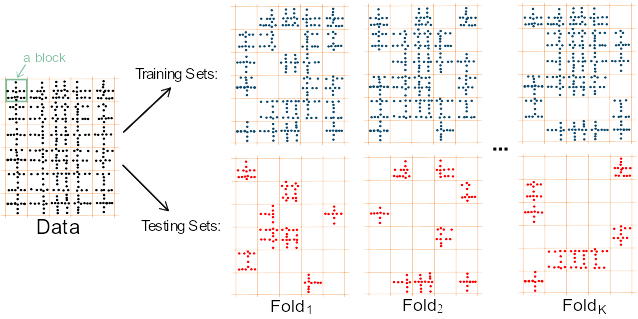
\includegraphics[width=1\linewidth]{paper/figures/bk_cv.png}
  \caption{
    The Block K-Fold Cross Validation method. The black dots are the data, the orange blocks are the non-overlapping spatial blocks of a specified size, the blue dots are the training sets for each iteration and the red dots are the testing sets for each fold.
    }
  \label{fig:BK-CV}
\end{figure}

The model accuracy can be assessed though the Root Mean Square Error (RMSE) calculated between the observed data from the testing set (\textcolor{orange}{$\mathbf{d^o_{test}}$}) and the predicted total-field anomaly also on the testing set coordinates (\textcolor{orange}{$\mathbf{d_{test}}$}):

\begin{equation}
    \label{eq:rmse}
    \text{RMSE}_k = \sqrt{\dfrac{\sum\limits_{i=1}^L \left(\textcolor{orange}{{d^o_{test_i}}} - \textcolor{orange}{{d_{test_i}}}\right)^2}{L}}
    \ ,
\end{equation}

\noindent
for $L$ number of testing points. This BK-CV process is iterated until all the folds have been used for both testing and training (see Figure~\ref{fig:BK-CV}). The overall BK-CV RMSE is determined by taking the average of all the $\text{RMSE}_k$ values across the folds. This BK-CV is summarised in Algorithm~\ref{alg:BK-CV}.

\begin{algorithm}[!h]
    \setstretch{1.5}
    Split the data into blocks of a given size
    \;
    Split the blocks randomly into K folds, with roughly the same number of data per fold
    \;
    \For{each fold $k$}{
        Assign fold $k$ to the testing set and the remaining folds to the training set
        \;
        Estimate the parameters \textcolor{teal}{$\bar{\mathbf{c}}_k$} using the data from the training set and Equation~\ref{eq:normal_equations} or the gradient-boosted equivalent sources method
        \;
        Predict the total-field anomaly \textcolor{orange}{$\Delta T (x, y, z)$} on the coordinates of the testing set using Equation~\ref{eq:tfa_eqs}
        \;
        Calculate the $\text{RMSE}_k$ between the observed data from the testing set (\textcolor{orange}{$\mathbf{d^{o}_{test}}$}) and the predicted total-field anomaly (\textcolor{orange}{$\mathbf{d_{test}}$}) using Equation~\ref{eq:rmse}
        \;
    }
    Calculate the BK-CV RMSE by taking the average of all the $\text{RMSE}_k$ calculated for each fold.
    \BlankLine
    \setstretch{1}
    \caption{The Block K-fold Cross-Validation method.}
    \label{alg:BK-CV}
\end{algorithm}

To determine the optimal hyper-parameters for each layer, a range of values for damping and relative depth is systematically generated. \citet{Dampney1969} suggests bounds of 2.5 to 6 times the average distance to the nearest neighbouring data points for the relative depth of equivalent sources. This range is utilised for the deep equivalent sources to ensure the regional long-wavelength signals are captured. For the shallow layer, a range of relative depths between the data heights and the deep layer are employed. Additionally, a range of $1 \times 10^{-10} \text{ to } 1 \times 10^{10}$ is used for the damping parameter $\mu$ (see Equation~\ref{eq:goal_function}). Once these ranges are defined, a comprehensive set of all the possible combinations of these hyper-parameters is created. For each combination, the BK-CV method (Algorithm~\ref{alg:BK-CV}) is employed to determine the corresponding BK-CV RMSE, which serves as the performance metric. The combination that yields the smallest BK-CV RMSE is then selected as the optimal set of parameters for the final equivalent source model.


%%%%%%%%%%%%%%%%%%%%%%%%%%%%%%%%%%%%%%%%%%%%%%%%%%%%%%%%%%%%%%%%%%%%%%%%%%%%%%%
\section{Synthetic Data Application}

To assess the accuracy of the interpolations, the method was applied to synthetic datasets containing magnetic sources with varying shapes, sizes, depths and induced magnetisations. To ensure consistency with real-world conditions, the synthetic dataset was simulated using the flight lines from the ICEGRAV 2013 aeromagnetic dataset \citep{ICEGRAV_data}, as detailed in Section~\ref{sec:real_application}. These flight line coordinates were projected using the Universal Polar Stereographic (UPS) projection, specifically for the South Pole region. The Earth's main magnetic field direction was set to match the IGRF orientation at the time of the original measurements, with an inclination of -65$^\circ$ and declination of 35$^\circ$, consistent with the real aeromagnetic dataset. A regional magnetic field was modelled using the ``checkerboard'' function of Verde  \citep{verde} on a regularly spaced grid covering the entire survey area, located at 60 km beneath the surface with an oscillating height of 15 km amplitude. The magnetisation for the regional field was specified to have an inclination of -50$^\circ$, declination of 40$^\circ$ and magnitude of $5 \times 10^{12}$Am$^2$. A zero-mean pseudo-random Gaussian noise, with a standard deviation of 5 nT, was also applied to the regional field. Additionally, a deep dipole was added to study the effects of a truncated long-wavelength signal (see Section~\ref{sec:truncated_regional} for further details). This dipole was placed at coordinates (2250 km, 2730 km, -70 km), with a magnetisation of 55$^\circ$ inclination, 45$^\circ$ declination and $2 \times 10^{13}$Am$^2$ magnitude. The descriptions of the shallower synthetic sources can be found in Table~\ref{table:shallow_sources}, in which the characteristics of their shape, location and magnetisation are outlined.

\begin{table}[tb!]
\centering
\begin{tabular}{c c c c c c}
\toprule
 &  & Centre Location (km) &  & Magnetisation & \\
\cmidrule{4-6}
Source & Type & [x, y, depth] & Inc ($^\circ$) & Dec ($^\circ$) & Magnitude (Am$^2$) \\
\midrule
1 & Oval & [1930, 3030, 6] & 75 & 60 & $2 \times 10^{10}$ \\
2 & Irregular & [1960, 2980, 0.8] & -60 & 45 & $3 \times 10^{9}$ \\
3 & Small Dipole & [1950, 2785, 0.5] & 45 & -65 & $5 \times 10^{10}$ \\
4 & Small Dipole	& [2100, 3011, 0.5] & 45 & -65 & $5 \times 10^{10}$ \\
5 & Small Dipole & [2110, 2955, 0.5] & 45 & -65 & $5 \times 10^{10}$ \\
6 & Small Dipole & [2150, 2750, 0.5] & 45 & -65 & $5 \times 10^{10}$ \\
7 &	Linear (Dyke) & [2200, 2950, 1] & -70 & 80 & $1 \times 10^{9}$ \\
8 & Linear (Dyke) & [2220, 2870, 5] & -70 & 80 & $2 \times 10^{9}$ \\
9 & Irregular & [2230, 2820, 0.9] & 50 & 70 & $5 \times 10^{9}$ \\
10 & Regional Dipole & [2260, 2830, 8] & -70 & 40 & $1 \times 10^{10}$ \\
\bottomrule
\end{tabular}
\caption{Descriptions of the shallower synthetic sources.}
\label{table:shallow_sources}
\end{table}

\subsection{Single and Dual Layer Comparison}
\label{sec:single_vs_dual}

\begin{figure}[tb!]
\centering
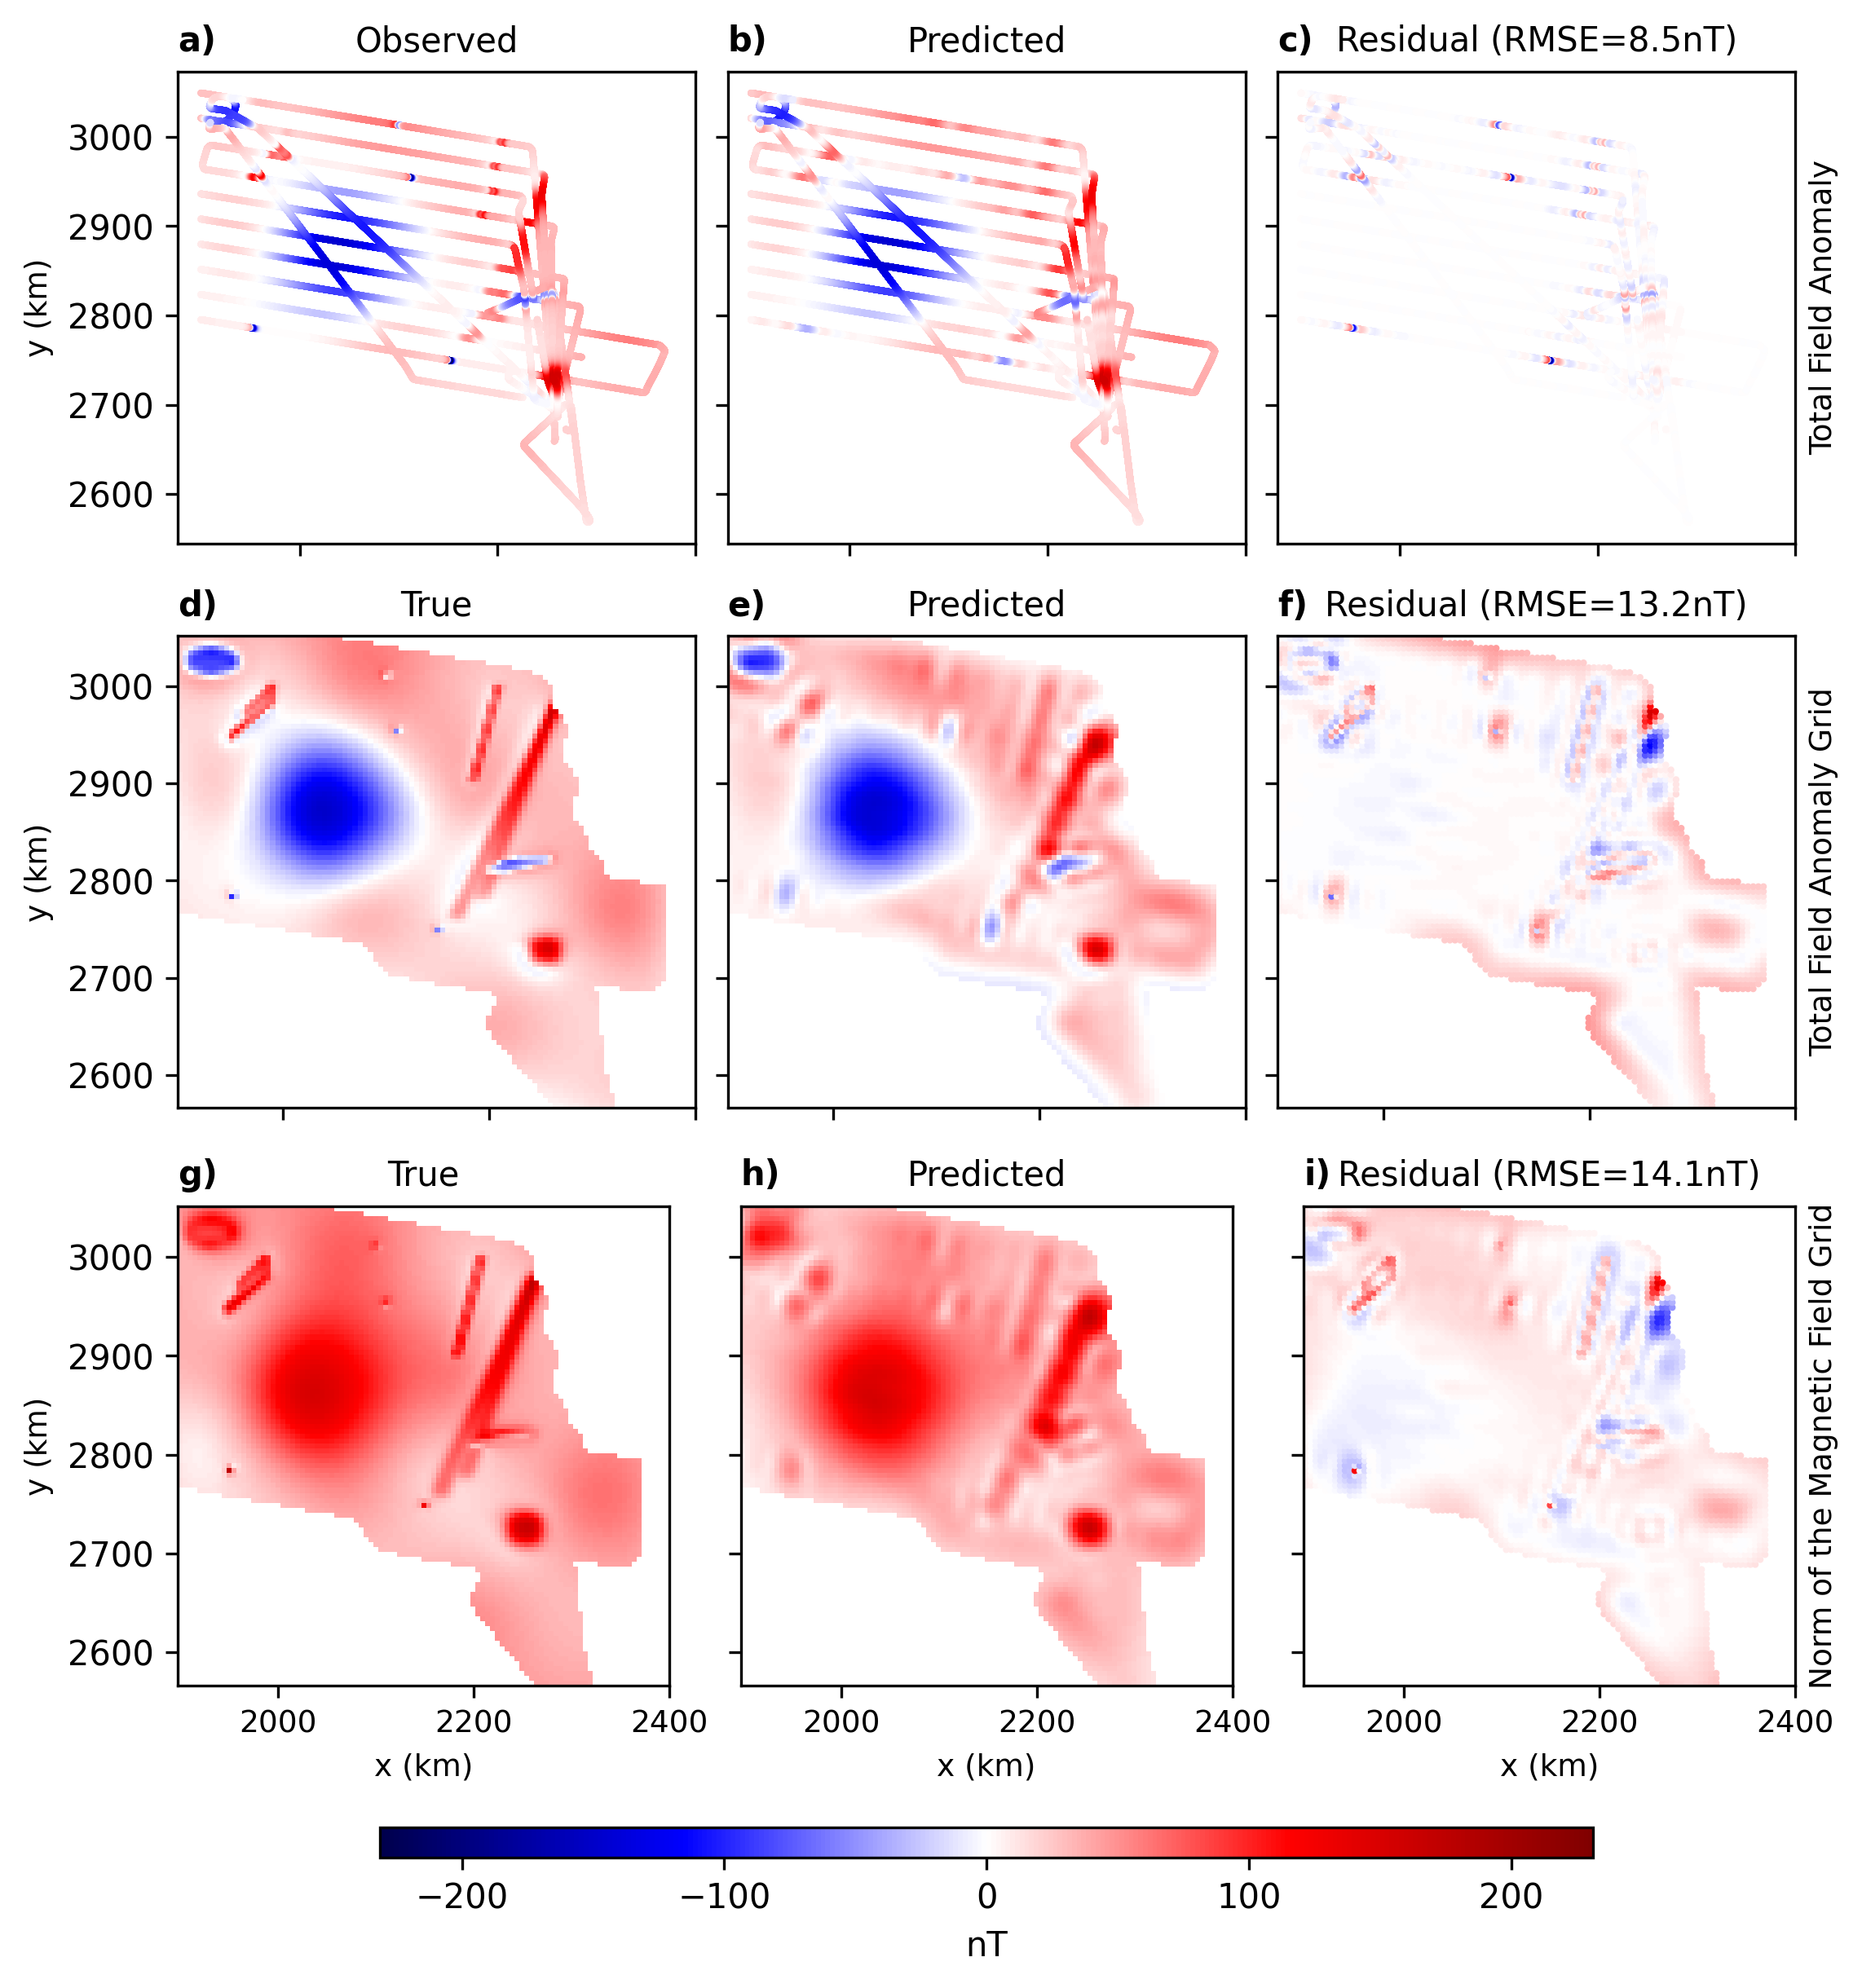
\includegraphics[width=1\linewidth]{figures/single_layer_synthetic.png}
\caption{
    Synthetic data and the predictions using a single layer of equivalent sources. a) observed total field anomaly of the synthetic data on the survey lines from the ICEGRAV survey \citep{ICEGRAV_data}, b) total field anomaly prediction on the survey lines, c) residual between the observed (a) and predicted (b) total field anomaly on the survey lines with a RMSE of 8.5 nT; d) true total field anomaly on a regular grid with 5 km spacing, e) predicted total field anomaly on regular grid with 5 km spacing, f) residual between the true (d) and predicted (e) total field anomaly on a regular grid with 5 km spacing and an RMSE of 13.2 nT; g) true norm of the anomalous magnetic field on a regular grid with 5 km spacing, h) predicted norm of the anomalous magnetic field on a regular grid with 5 km spacing, i) residual between the true (g) and predicted (h) norm of the anomalous magnetic field on a regular grid with 5 km spacing and an RMSE of 14.1 nT.
}
\label{fig:single_layer_synthetic}
\end{figure}

\begin{figure}[tb!]
\centering
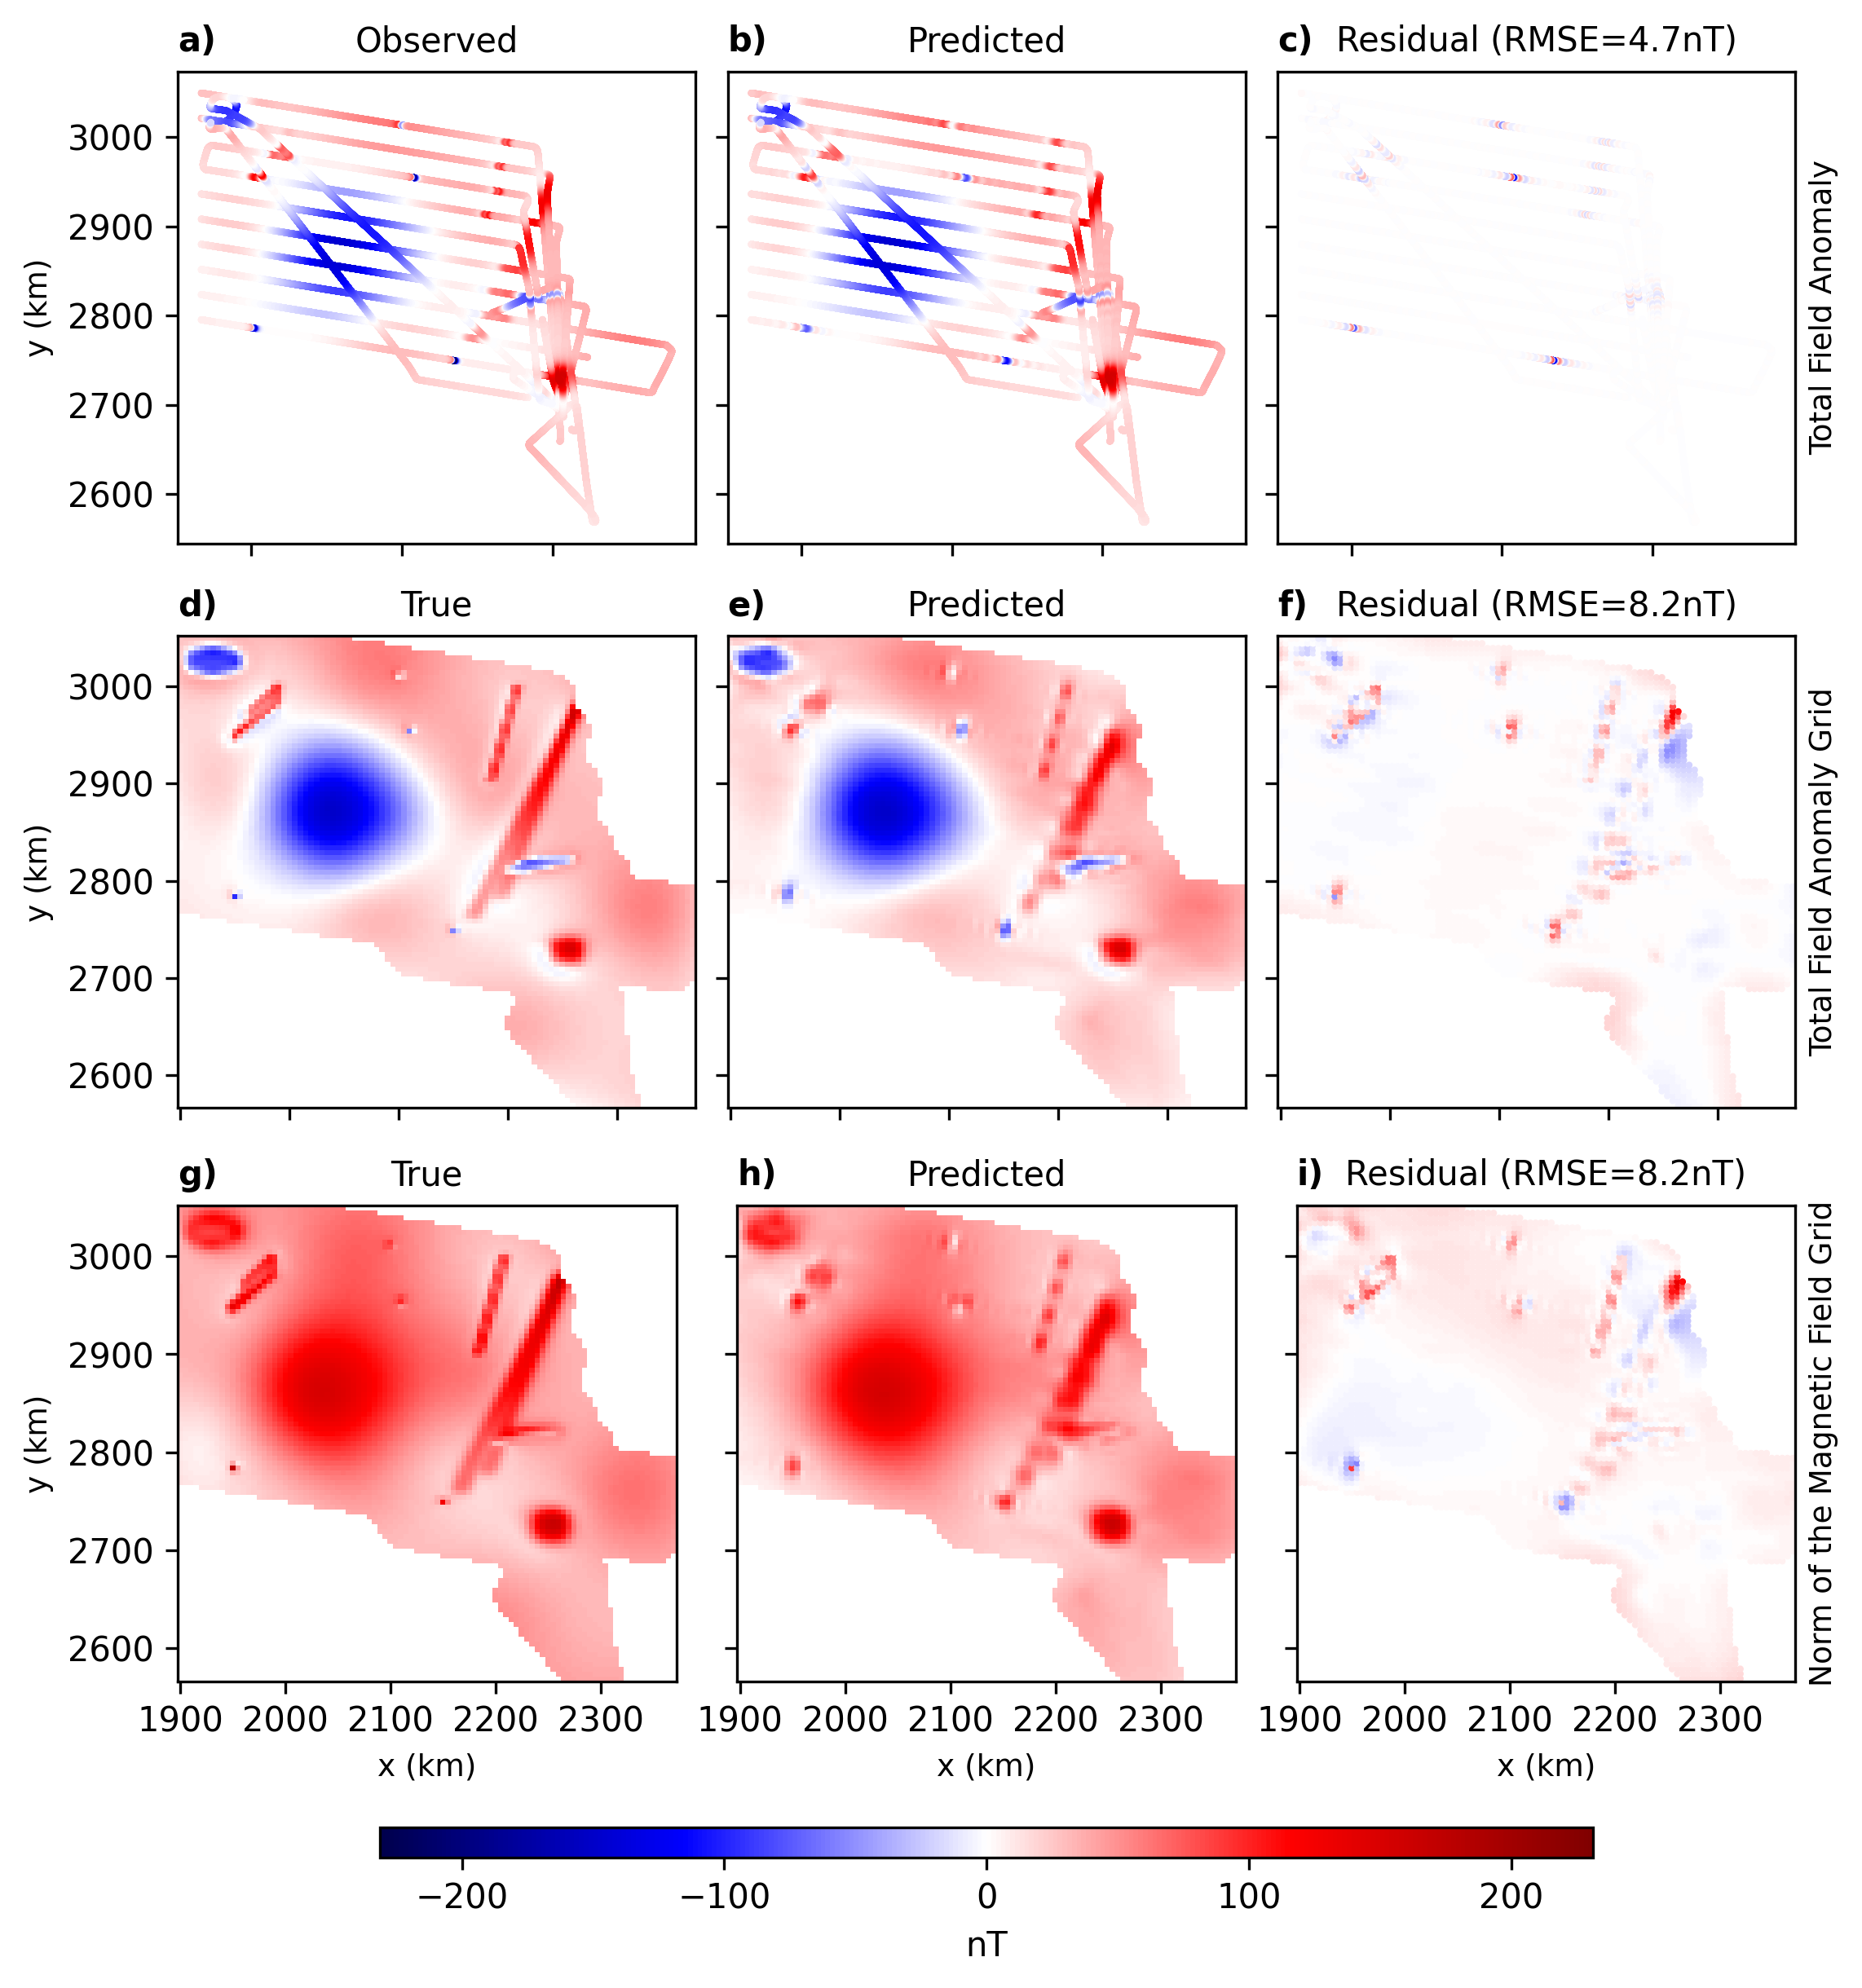
\includegraphics[width=1\linewidth]{figures/dual_layer_synthetic.png}
\caption{
    Synthetic data and the predictions using the dual layer equivalent sources. a) observed total field anomaly of the synthetic data on the survey lines from the ICEGRAV survey \citep{ICEGRAV_data}, b) total field anomaly prediction on the survey lines, c) residual between the observed (a) and predicted (b) total field anomaly on the survey lines with a RMSE of 4.7 nT; d) true total field anomaly on a regular grid with 5 km spacing, e) predicted total field anomaly on regular grid with 5 km spacing, f) residual between the true (d) and predicted (e) total field anomaly on a regular grid with 5 km spacing and an RMSE of 8.2 nT; g) true norm of the anomalous magnetic field on a regular grid with 5 km spacing, h) predicted norm of the anomalous magnetic field on a regular grid with 5 km spacing, i) residual between the true (g) and predicted (h) norm of the anomalous magnetic field on a regular grid with 5 km spacing and an RMSE of 8.2 nT.
}
\label{fig:dual_layer_synthetic}
\end{figure}

To assess the performance of a single versus a dual layer of equivalent sources, the single layer of equivalent sources was first applied using the GB EQS method (see Algorithm~\ref{alg:gradient_boosting}). To ensure optimal selection of the hyper-parameters, the BK-CV method (see Algorithm~\ref{alg:BK-CV}) was employed, using a block size of 30 km $\times$ 30 km over a wide range of parameter values. The optimal hyper-parameters, which resulted in the lowest BK-CV RMSE, were a damping value of $1 \times 10^{2}$ and a relative depth of 35km. With these optimised parameters, the GB EQS method (see Algorithm~\ref{alg:gradient_boosting}) was applied using a window size of 250 km $\times$ 250 km. To minimise errors in the initially selected windows of the iteration, the method was repeated twice. 

The resulting single-layer predictions for the total field anomaly along the survey lines, total field anomaly on the regular grid, and the norm of the anomalous magnetic field on the regular grid are presented in Figure~\ref{fig:single_layer_synthetic}. The prediction of the total field anomaly along the survey lines (Figure~\ref{fig:single_layer_synthetic}b) provides overall an accurate prediction, with an RMSE of 8.5nT. However, it underestimates the magnitude of the four small, shallow dipoles, a pattern consistent with the predictions for both, the total field anomaly (Figure~\ref{fig:single_layer_synthetic}e) and the norm of the anomalous magnetic field (Figure~\ref{fig:single_layer_synthetic}h) on a regular grid. Furthermore, the single layer model introduces undulating ripple effects at the edges of the sources, especially along the dykes. It also generates edges effects at the borders of the survey area. These results highlight a key challenge when fitting both, the long-wavelength components and the short-wavelength components simultaneously with a single layer.

Further exploration of the single layer model reveals an inherent trade-off: when placing the equivalent source layer deeper, it captures the regional, long-wavelength signals more effectively but struggles with the short-wavelength signals. Conversely, placing the equivalent source layer shallower, improves the capture of the short-wavelength signals but compromises the ability to determine the regional, long-wavelength signals. This balancing act emphasises the limitations of using a single-layer approach in modelling multi-scale sources and underlines the need for using a multi-layer model.

To explore the potential benefits of a dual layer model, the dual layer equivalent source method (see Algorithm~\ref{alg:dual_layer}) was applied. The observed data was block averaged using different block spacings in order to determine the ideal size that isolates the long-wavelength signals for the deep layer to fit. When the block spacing is too small, some of the short-wavelength signals are captured, resulting in the deep layer not capturing all of the regional, long-wavelength signals due to trying to fit both long- and short-wavelengths. When the block spacing is too large, not all of the regional signals are captured either. Those chosen ideal block spacing for this synthetic data was 25 km $\times$ 25 km with a padding of $0.2 \times $ block spacing. The use of padding allows for more data points that fall along the survey boundary to be used, reducing the potential for edge effects at the borders that were seen in the single layer model. Using the BK-CV method (see Algorithm~\ref{alg:BK-CV}) with a block size of 100 km $\times$ 100 km, the optimal hyper-parameters for the deep layer, which resulted in the lowest BK-CV RMSE, were a damping value of 1 and a relative depth of approximately 117 km ($6 \times$ grid spacing). The shallow layer was then fitted to the residuals from the deep layer in order to focus on fitting the shorter-wavelength signals, as well as correct potential errors caused by the deep layer. The GB EQS method (see Algorithm~\ref{alg:gradient_boosting}) was utilised with a window size of 250 km $\times$ 250 km, matching the single layer model. To optimise the shallow layer’s hyper-parameters, the BK-CV method was applied with a block size of 30 km $\times$ 30 km (the same as the single layer model) to account for local variations in the data. The optimal hyper-parameters for the shallow layer, resulting in the lowest BK-CV RMSE, were a damping value of $1 \times 10^{2}$ and a relative depth of 17 km. The GB EQS method (see Algorithm~\ref{alg:gradient_boosting}) was applied twice to the shallow layer to minimise potential errors in the initial windows selected in the iteration, similar to the single layer model. 

The dual-layer EQS results for the total field anomaly along the survey lines, regular grid, and the norm of the anomalous magnetic field on the regular grid are shown in Figure~\ref{fig:dual_layer_synthetic}. The dual layer model provides a significantly improved prediction of the total field anomaly along the survey lines (Figure~\ref{fig:dual_layer_synthetic} b), with an RMSE of 4.7nT, particularly in capturing the four small dipoles. It also demonstrates the method is able to interpolate onto regularly gridded lines and upward continue to a constant height (see Figure~\ref{fig:dual_layer_synthetic} e and h). Additionally, the regional field prediction is much smoother, with no edge effects at the survey borders or along the dykes, for both the total field anomaly and norm of the anomalous magnetic field. This will allow different surveys to be blended more easily. The dual layer model successfully reduces the undulating ripple effects near the edges of the sources. However, the dual-layer method does face challenges when predicting on the regular grid (Figure~\ref{fig:dual_layer_synthetic} e and h). Specifically, the method struggles with artifacts related to the flight lines, particularly along the dykes. The gaps between the survey lines appear more pronounced in these areas, leading to visible discontinuities. This issue could be addressed by adjusting the relative depth of the shallow layer, but in doing so may impact the accuracy of the small anomalies such as the small dipoles. Therefore, after using the Block K-Fold Cross Validation to narrow the range of optimal values, visual inspection of the predictions is necessary in order to select the final value.

Overall, the dual-layer approach improves predictions, for both total field anomaly and norm of the anomalous magnetic field, by allowing the deep layer to capture the regional, long-wavelength signals, whilst the shallow layer focuses on the short-wavelength signals and corrects potential errors from the deep layer. This combination enhances the accuracy when compared to the single-layer approach, illustrating the advantages of using multiple layers of equivalent sources to model multi-scale sources. Applying padding to the deep layer reduces the edge effects along the survey borders, a common artefact when using a single layer model. The BK-CV method provides a more automated and efficient way to select optimal hyper-parameters. Additionally, the use of the GB EQS method reduces the computational load and the processing time. By repeating this method twice also helps to minimise errors in the initial selection of windows during the iteration.

\subsection{Truncated Long-wavelength Anomaly}
\label{sec:truncated_regional}

\begin{figure}[tb!]
\centering
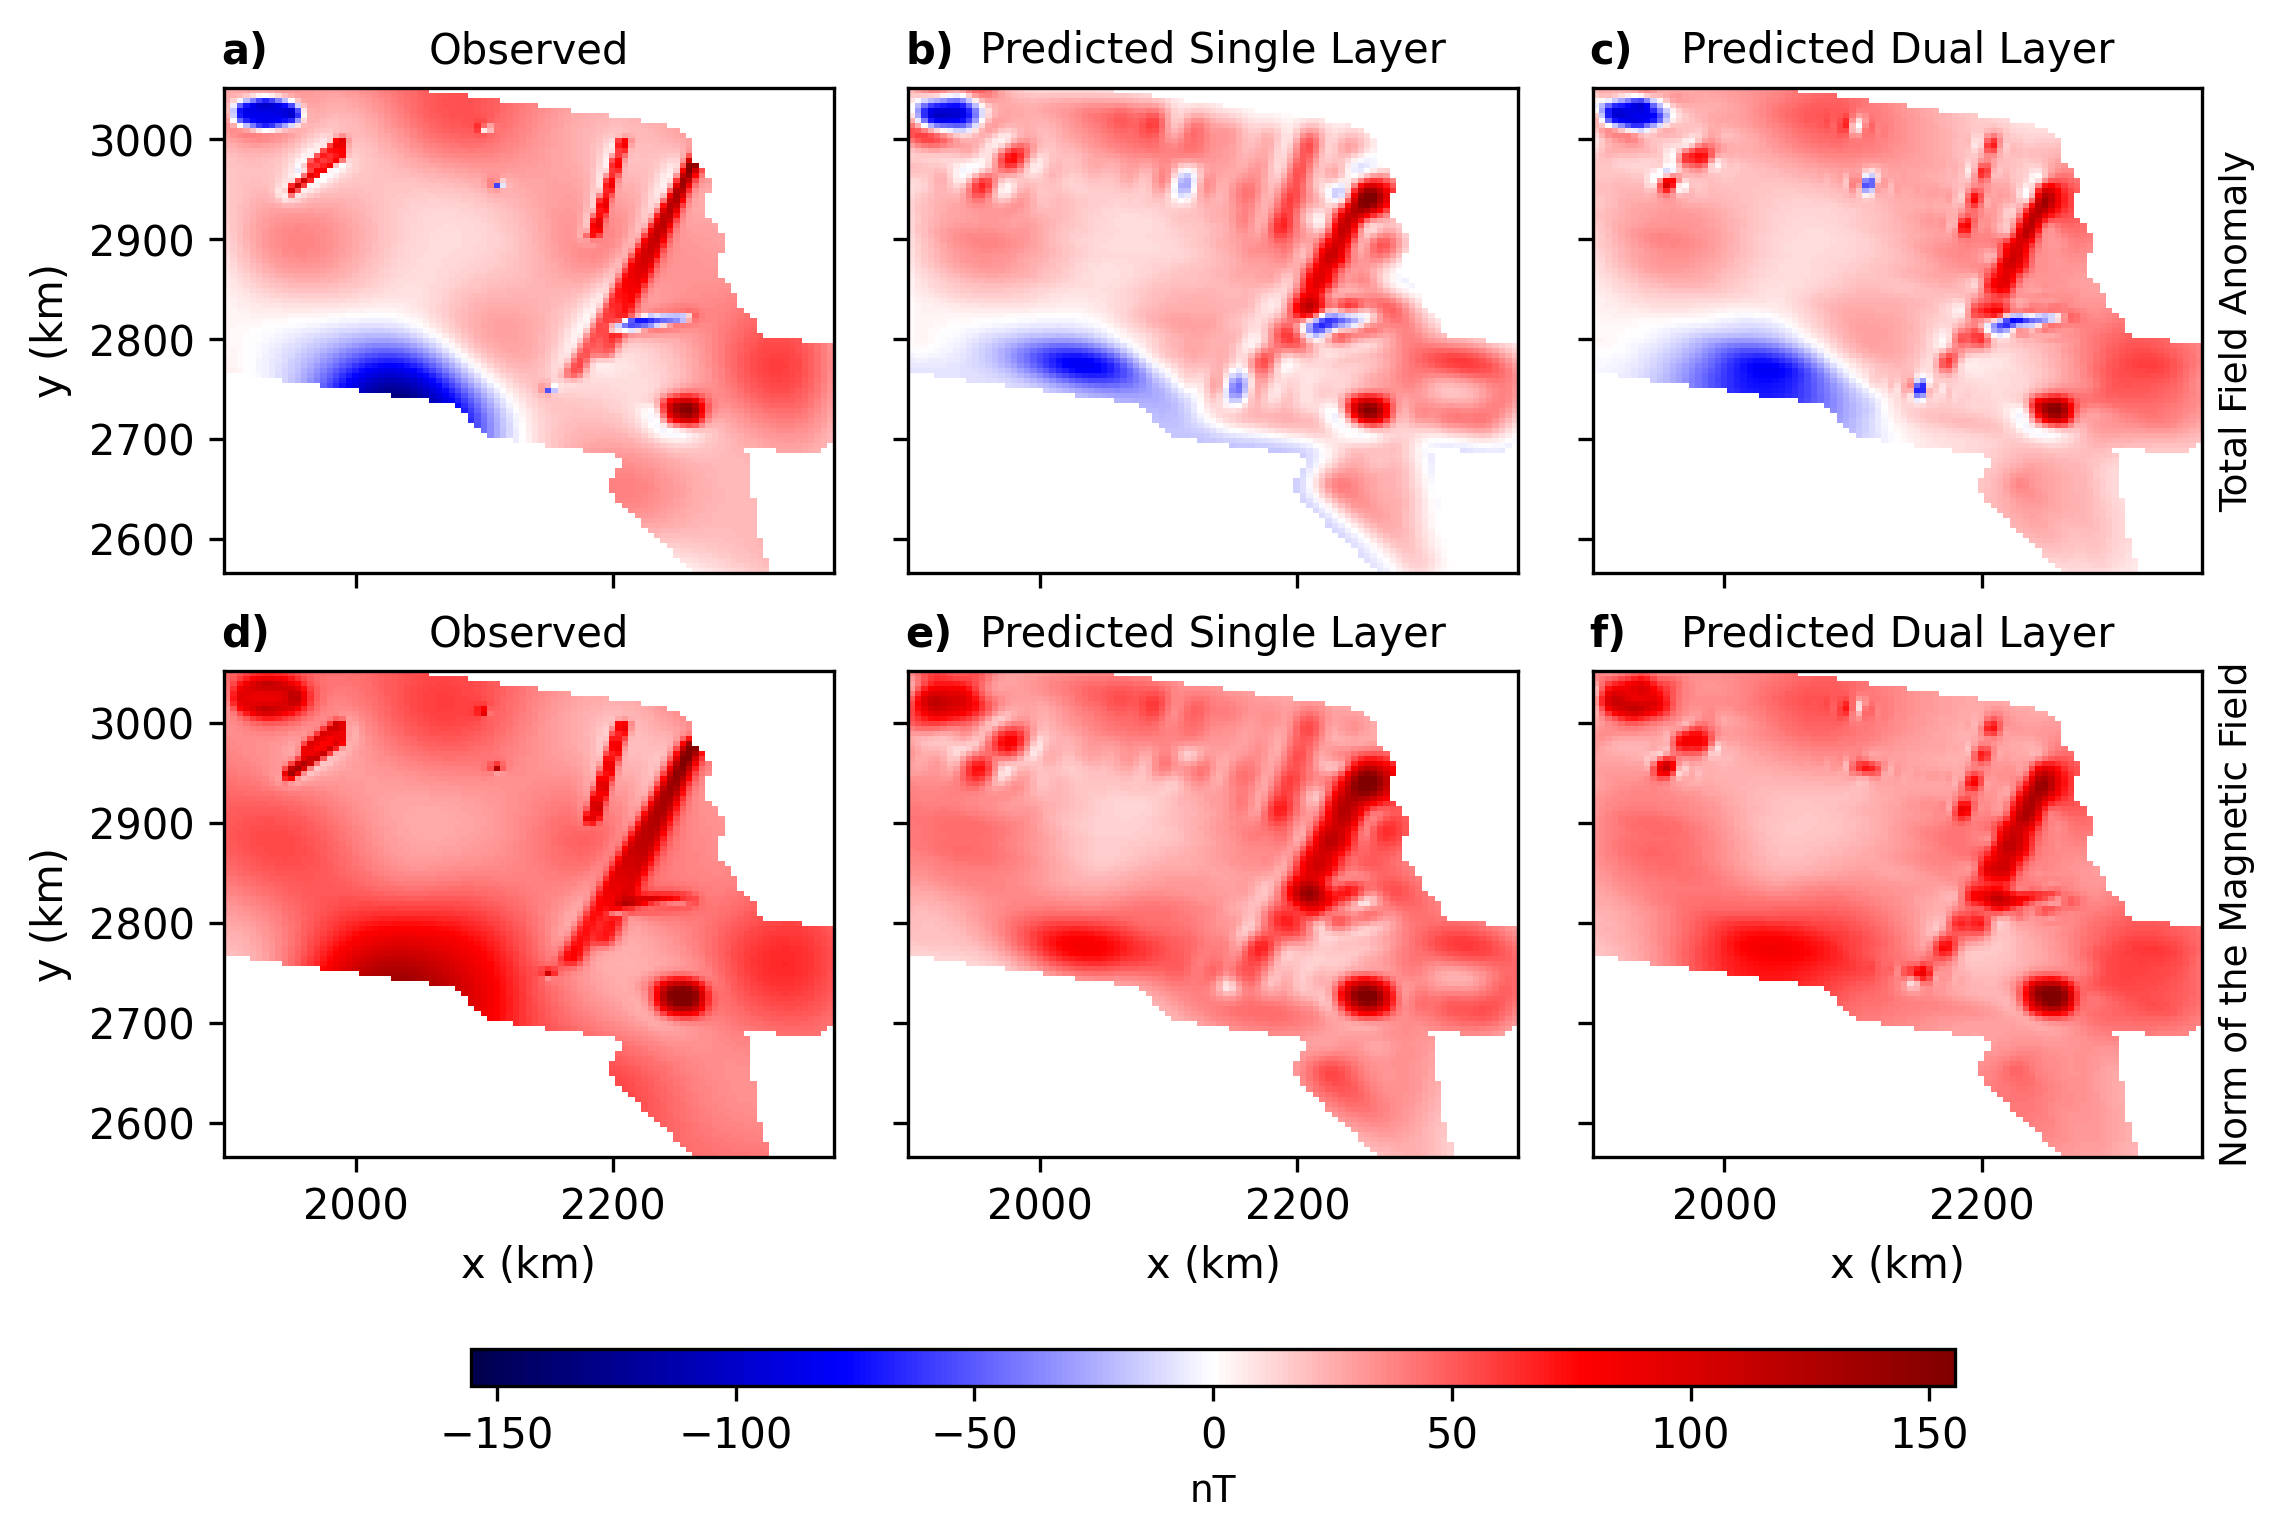
\includegraphics[width=1\linewidth]{paper/figures/truncated_regional.png}
\caption{
    Synthetic data with a truncating regional dipole and the predictions using a single and dual layer of equivalent sources. a) true total field anomaly on a regular grid with 5km spacing, b) predicted total field anomaly on regular grid with 5km spacing using a single layer of equivalent sources, c) predicted total field anomaly on a regular grid with 5km spacing using the dual layer of equivalent sources; d) true norm of the anomalous magnetic field on a regular grid with 5km spacing, e) predicted norm of the anomalous magnetic field on a regular grid with 5km spacing using a single layer of equivalent sources, c) predicted norm of the anomalous magnetic field on a regular grid with 5km spacing using the dual layer of equivalent sources.
}
\label{fig:truncated_regional}
\end{figure}

\begin{figure}[tb!]
\centering
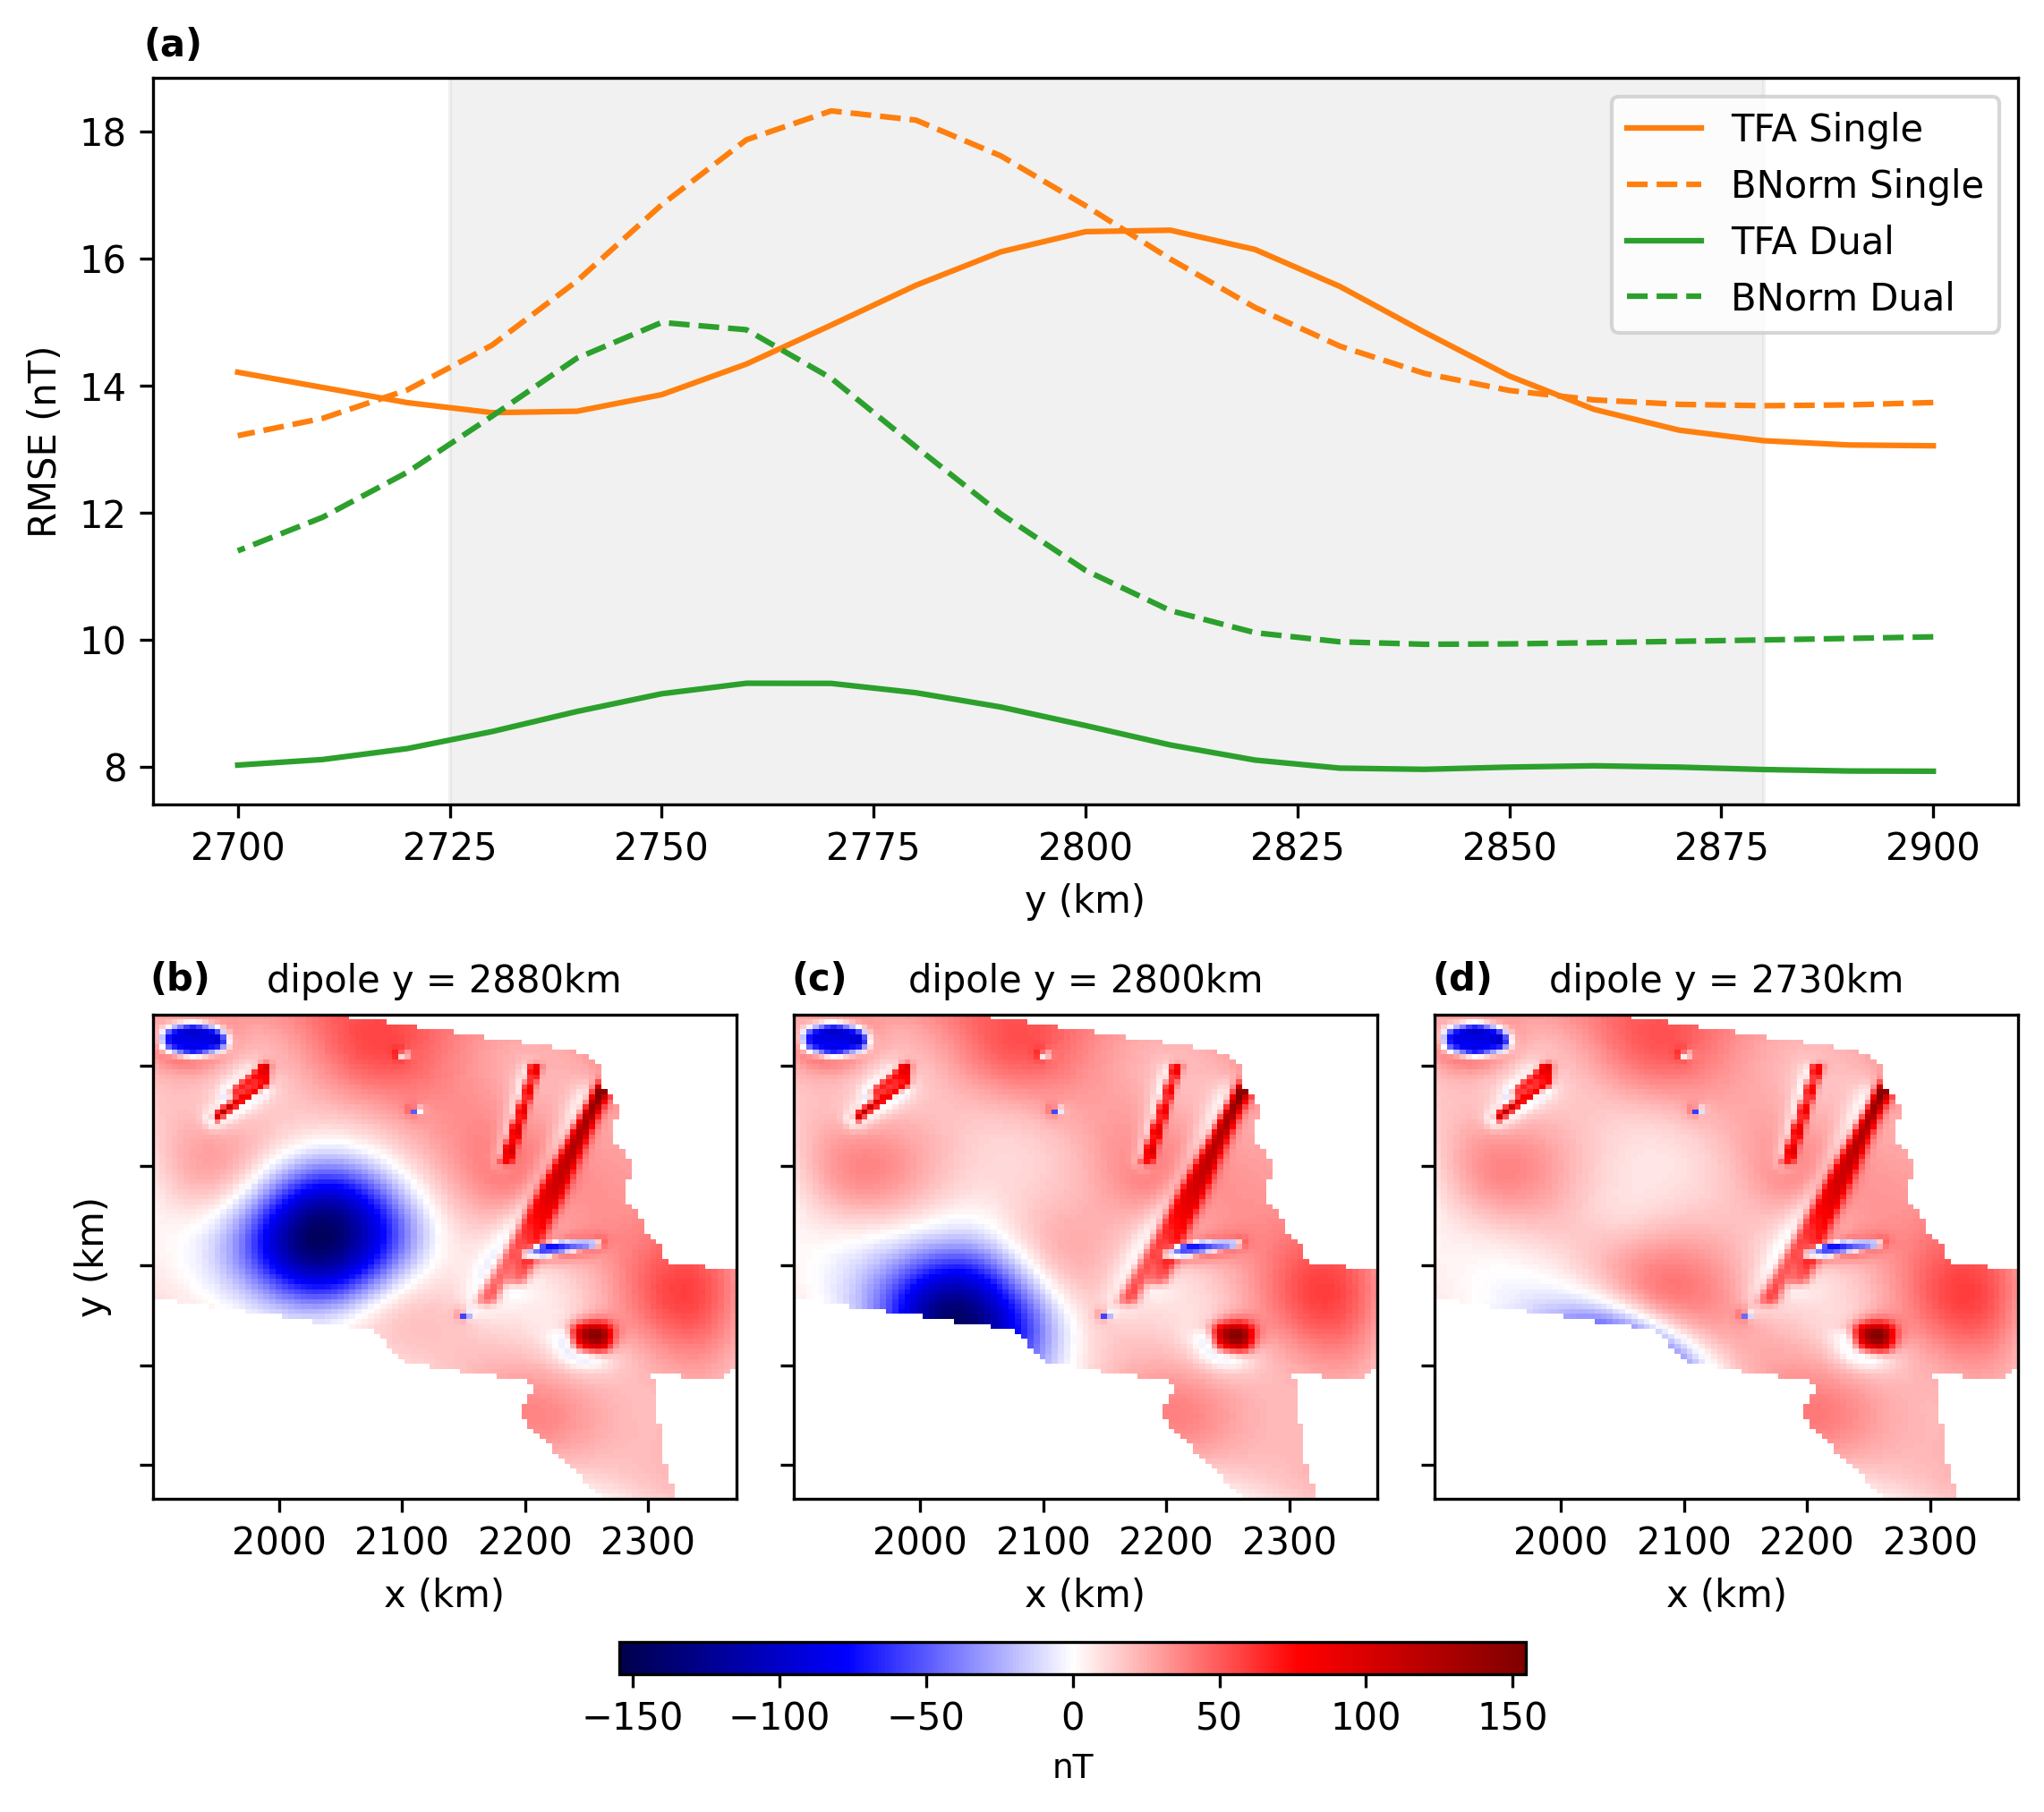
\includegraphics[width=1\linewidth]{paper/figures/truncated_regional_rmses.png}
\caption{
    The Root Mean Square Error (RMSE) from the predictions of the total field anomaly (solid lines) and norm of the anomalous magnetic field (dashed lines) on a regular grid (with 5km spacing) as the regional dipole was shifted outside the survey boundary (a). The x-axis in (a) shows the y-coordinate at the top of the regional dipole. The RMSEs from the single-layer approach are shown in orange and the RMSEs from the dual-layer approach are shown in green. The shaded grey region in (a) highlights when the regional dipole was truncated and could partially be seen within the survey bounds. (b-d) shows the true total field anomaly on regular grids (with 5km spacing) with the regional dipole located at different y-coordinates as it was shifted outside the survey bounds. The y-coordinates at the top of the regional dipole are 2730km (b), 2800km (c) and 2880km (d).
}
\label{fig:truncated_regional_rmses}
\end{figure}

The impact of a truncated long-wavelength signal was also investigated further after observing the single-layer approach struggled to accurately predict the regional field. To assess this effect, both the single and dual layer models were applied while progressively truncating the regional dipole by moving it beyond the survey boundary. An example of the truncated regional dipole is illustrated in Figure~\ref{fig:truncated_regional}). Both single- and dual-layer approaches appear to underestimate the magnitude of the truncated regional signal. Furthermore, the single-layer approach creates edge effects along the survey bounds resulting from the truncated regional signal (see Figure~\ref{fig:truncated_regional}b). On the contrary, the dual-layer approach mitigated these edge effects (see Figure~\ref{fig:truncated_regional}c), which was also noted in Section~\ref{sec:single_vs_dual}.

As the regional dipole became increasingly truncated, the RMSE for both models increased and then decreased back to the initial RMSE as the dipole influence became less visible. The RMSE for the norm of the anomalous magnetic field (see the grey shaded region of Figure~\ref{fig:truncated_regional_rmses}) significantly increased in comparison to the total field anomaly. The dual-layer approach consistently exhibited a lower RMSE compared to the single-layer approach, suggesting it provides more reliable predictions overall, as well as, in the presence of a truncated regional field signal. The impact of a truncated long-wavelength signal further highlights the importance of using a multi-layer approach when applying the equivalent sources technique.


%%%%%%%%%%%%%%%%%%%%%%%%%%%%%%%%%%%%%%%%%%%%%%%%%%%%%%%%%%%%%%%%%%%%%%%%%%%%%%%
\section{Real Data Application}
\label{sec:real_application}

\begin{figure}[tb!]
\centering
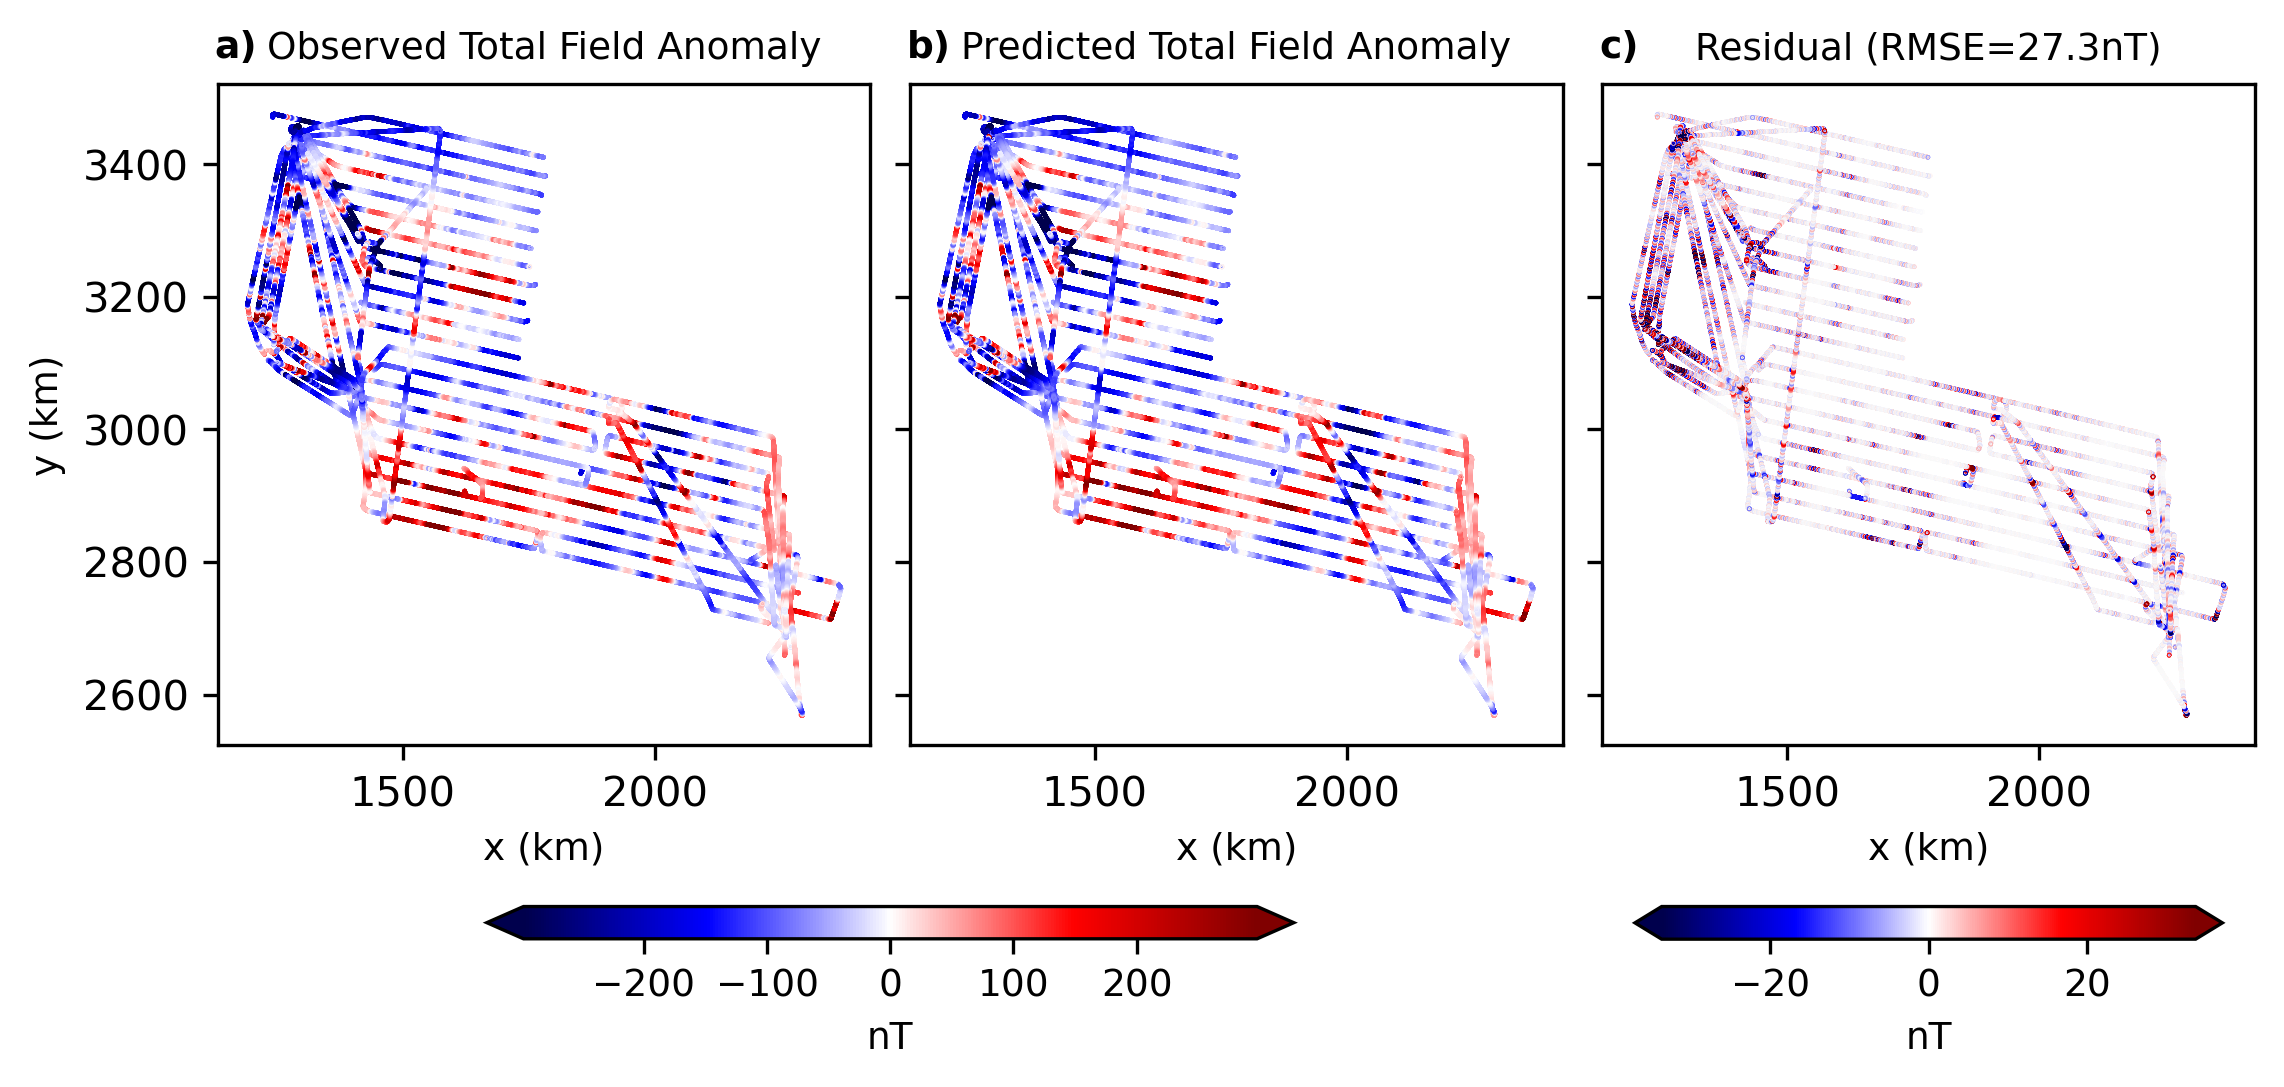
\includegraphics[width=1\linewidth]{paper/figures/real_line_pred.png}
\caption{
    The real data and prediction on the flight lines using the dual-layer approach. The observed total field anomaly data of the ICEGRAV survey \citep{ICEGRAV_data} (a), the prediction (b) on the same survey lines using the dual layer of equivalent sources and the residual (c) between the observed and the predicted with an RMSE of 27.3nT.
}
\label{fig:real_line_pred}
\end{figure}

The method was applied to the open-access aeromagnetic survey data from the ICEGRAV campaigns \citep{ICEGRAV_data}, which spanned from 2010 to 2013. The data covers parts of interior East Antarctica and the Antarctic Peninsula, including key areas such as the Dronning Maud Land ice stream systems and the Recovery Lakes drainage basin. This dataset was selected to showcase the effectiveness of the method on real-world data that features irregular survey flight lines, substantial spacing between those lines and varying line altitudes. The dataset’s distinctive characteristics, in terms of its vast geographical coverage, complex data collection and large amount of data points (404,363 data points), provide a robust and challenging test case for evaluating the method's performance in complex conditions.

\begin{figure}[tb!]
\centering
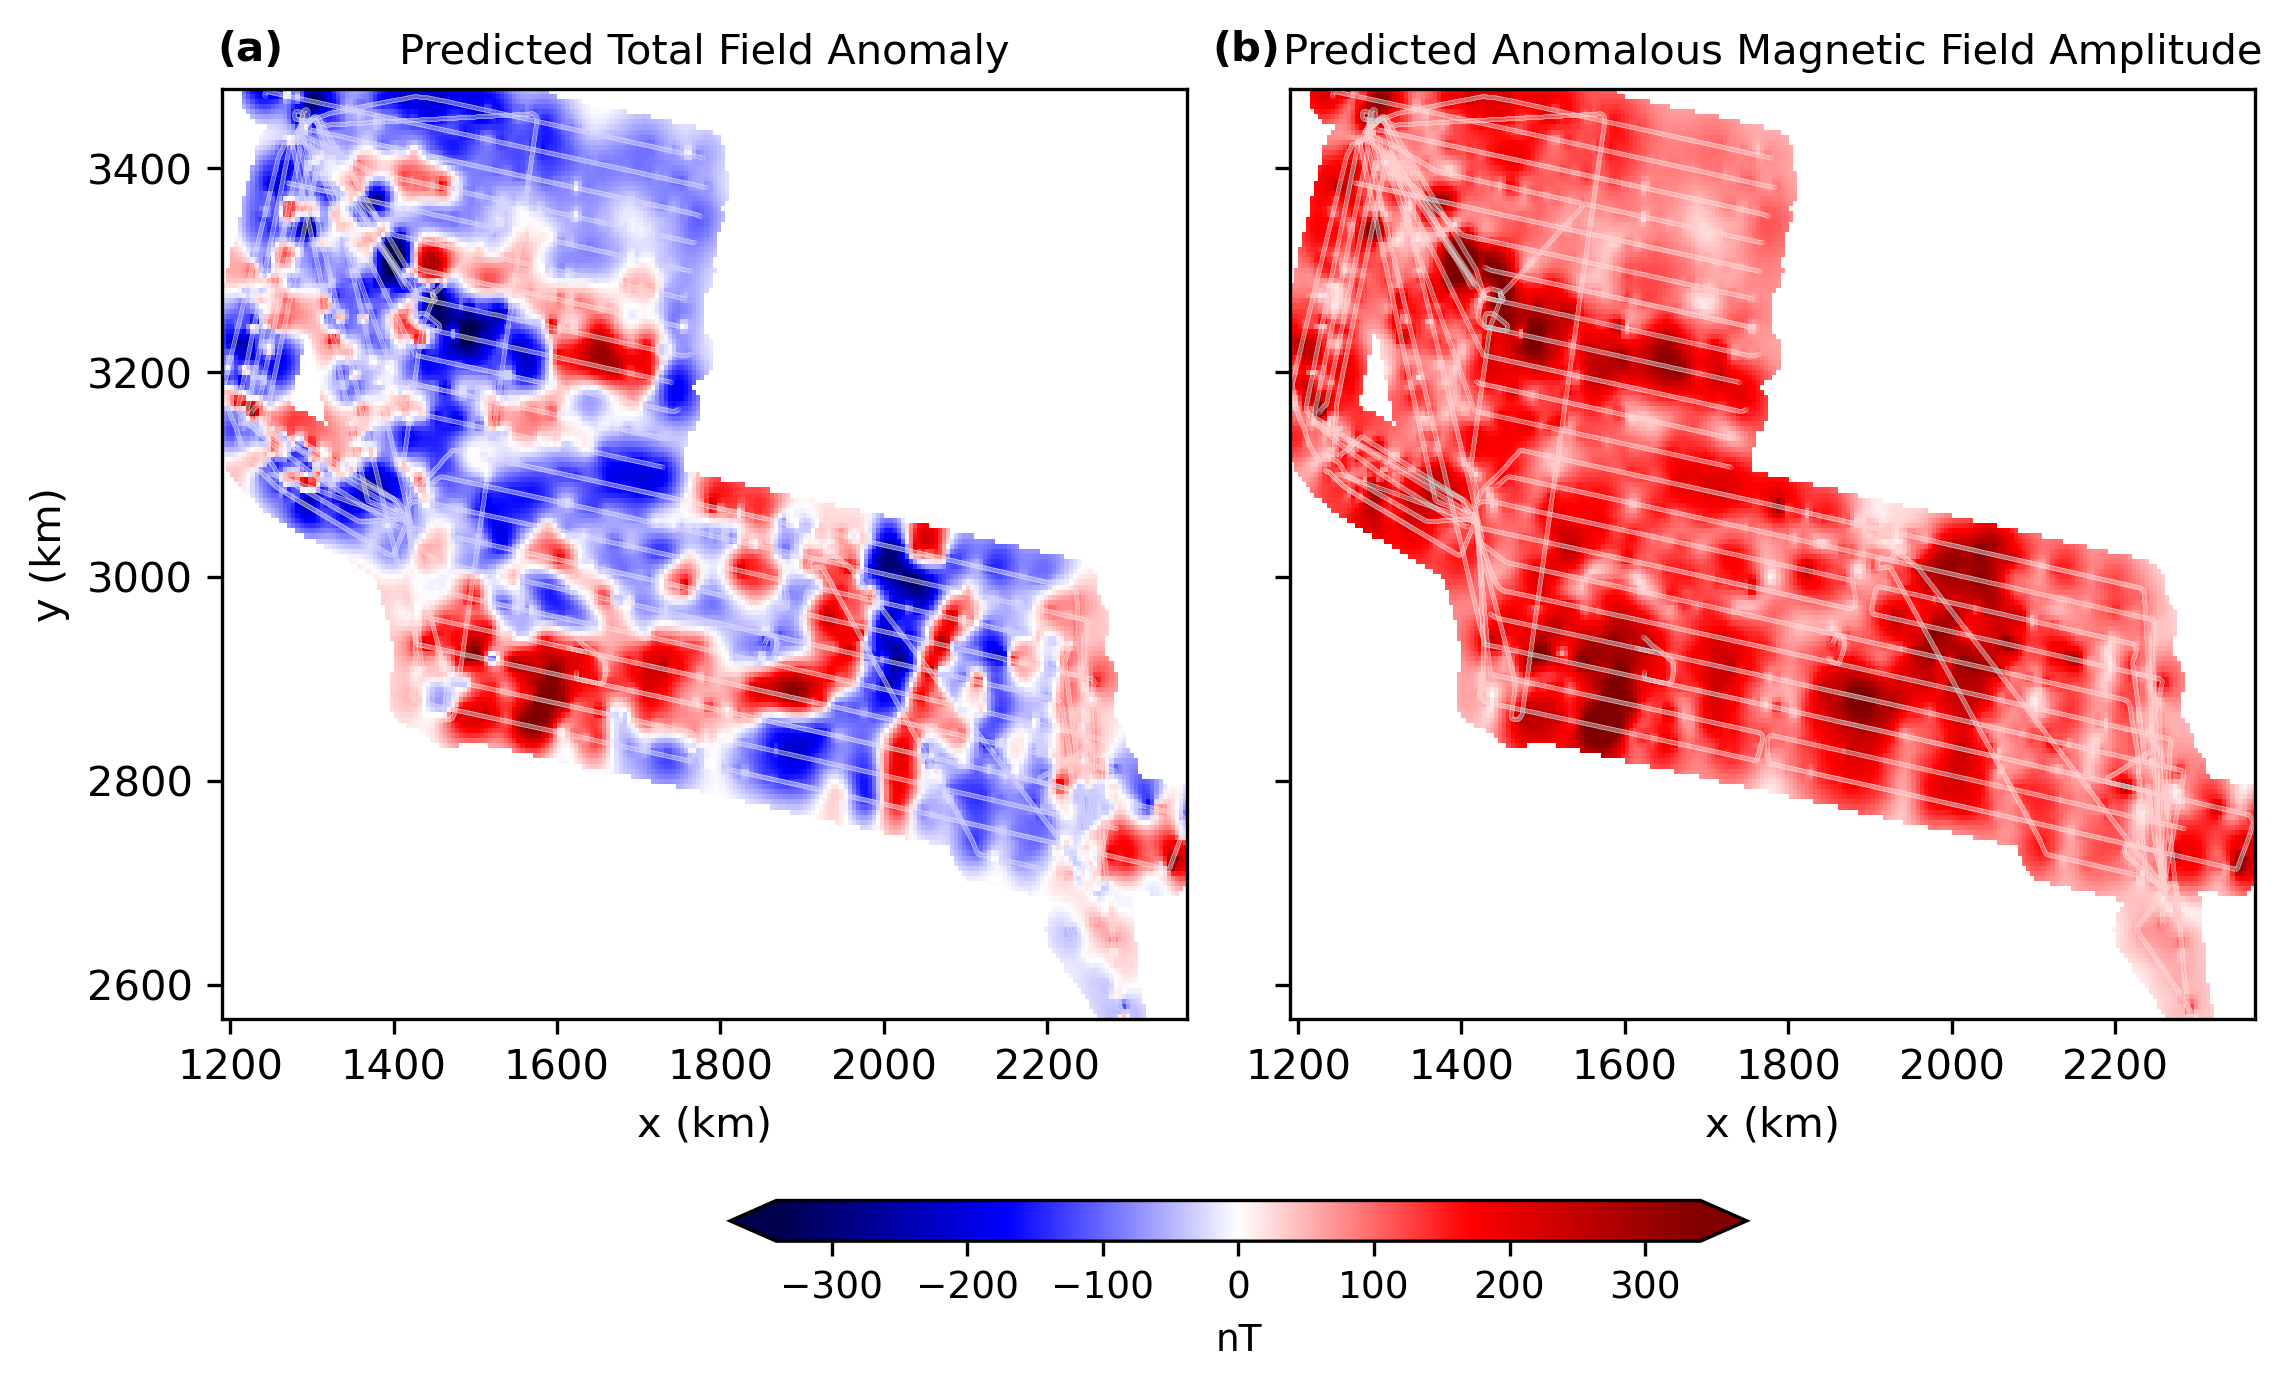
\includegraphics[width=1\linewidth]{paper/figures/real_grid_pred.png}
\caption{
    The real data predictions on a regular grid using the dual-layer approach. The prediction of the total field anomaly (a) and norm of the anomalous magnetic field (b) of the ICEGRAV survey \citep{ICEGRAV_data} on a regular grid with 5km spacing. The survey lines are shown in white.
}
\label{fig:real_grid_pred}
\end{figure}

The coordinates of this dataset were first projected using the Universal Polar Stereographic (UPS) projection, specifically for the South Pole region. The dual layer equivalent source method (see Algorithm~\ref{alg:dual_layer}) could then be applied to the observed data, which has already undergone preprocessing \citep{ICEGRAV_data}. To fit the deep equivalent source layer, the observed data was block-averaged using different block spacings to determine the ideal size for isolating most of the long-wavelength signals. A block spacing of 15 km $\times$ 15 km, with a padding of $ 0.3 \times $ the block spacing, was selected. The padding allows for additional data points along the survey boundary, reducing the potential for edge effects at the borders. The BK-CV method (see Algorithm~\ref{alg:BK-CV}) was applied with a block size of 200 km $\times$ 200 km to determine the optimal hyper-parameters which yield the lowest BK-CV RMSE. The chosen parameters were a damping value of 10 and a relative depth of approximately 55 km. The shallow layer was then fitted to the residuals from the deep layer using the GB EQS method (see Algorithm~\ref{alg:gradient_boosting}) with a window size of 400 km $\times$ 400 km. The BK-CV method (see Algorithm~\ref{alg:BK-CV}) was utilised again to determine the optimal hyper-parameters for the shallow layer. Using a block size of 20 km $\times$ 20 km, the chosen parameters with the lowest BK-CV RMSE were a damping value of 100 and a relative depth of approximately 10 km. The GB EQS method (see Algorithm~\ref{alg:gradient_boosting}) was applied twice to the shallow layer to minimise potential errors in the initially selected windows of the iterations. The results for the total field anomaly along the survey lines are shown in Figure~\ref{fig:real_line_pred}. The dual layer provides a good prediction of the complicated dataset, with an RMSE of 27.3nT.

The predictions of the total field anomaly and norm of the anomalous magnetic field on a regular grid are shown in Figure~\ref{fig:real_grid_pred}. Using a machine with 125 Gigabytes RAM, the dual layer approach took approximately 1 minute and 42 seconds to fit the observed total field anomaly and predict the norm of the anomalous field. Here, the method demonstrates its ability to interpolate onto regularly gridded lines, as well as upward continue to a constant height. The grid predictions reveal numerous points with magnitude close to 0nT, a pattern that is also present in the observed data. However, it remains uncertain whether these near-zero values represent real values or if they are artifacts introduced during the data preprocessing. If the latter is the case, more careful preprocessing is necessary before applying the equivalent source method.



%%%%%%%%%%%%%%%%%%%%%%%%%%%%%%%%%%%%%%%%%%%%%%%%%%%%%%%%%%%%%%%%%%%%%%%%%%%%%%%
\section{Conclusion}

Different adaptations of the Equivalent Source Technique have been developed to improve the computational efficiency and accuracy of the predictions. However, many of these approaches still face challenges, such as the need for regularly gridded data at constant height, reliance on a stabilising parameter or the presence of border effects in the predictions. The Dual-Layer Gradient-Boosted Equivalent Sources tackles these limitations by: 

\begin{enumerate}
    \item Using the dual-layer approach to improve the accuracy of the predictions and reduce the border effect.
    \item Use block-averaging and the Gradient-Boosted Equivalent Sources method to reduce the computational load.
    \item Apply Block K-Fold Cross Validation to guide optimal parameter selection for the model.
\end{enumerate}

The synthetic data tests demonstrate the dual-layer approach enhances the prediction accuracy by allowing the deeper layer to capture the regional, long-wavelength signals, whilst the shallower layer focuses on the short-wavelength signals. This approach also significantly improves predictions in cases where long-wavelength signals are truncated. Block-averaging the observed data reduces the number of sources needed in the deep layer, enabling it to focus on fitting the regional signals and decreasing the computational load. Applying padding to the deeper layer increases the number of data points along the survey border, reducing the potential for edge effects, a common issue with the Equivalent Source Technique. 
To further enhance the computation efficiency, the Gradient-Boosted Equivalent Sources technique was utilised for fitting the shallow layer. This approach solves several smaller damp least-squares problems rather than solve one large problem. Repeating the window iterations of the shallow layer twice helped to minimise errors in the initially selected windows.

The use of Block K-Fold Cross Validation has proven beneficial in narrowing the optimal range for the model hyper-parameters. However, visual inspection of the predictions still remains necessary to refine the final selection. This is due to the Equivalent Source Technique sometimes imprinting survey line artifacts onto the regular grid prediction.

Applying the Dual-Layer Gradient-Boosted Equivalent Sources to the ICEGRAV data demonstrated the method’s ability to successfully interpolate and upward continue the data on to a regular grid at a constant height, as well as predict the norm of the anomalous magnetic field. However, any artefacts from the data preprocessing will still be present in the final predictions, emphasising the importance of careful preprocessing before applying the method.


%%%%%%%%%%%%%%%%%%%%%%%%%%%%%%%%%%%%%%%%%%%%%%%%%%%%%%%%%%%%%%%%%%%%%%%%%%%%%%%
\section{Data Availability Statement}

The Python source code used to produce all of the results and figures presented here are available at \url{https://github.com/\GitHubRepository} and
\url{https://doi.org/\ArchiveDOI} under the CC-BY license and the MIT open-source license. This study also made use of the following open-source scientific software: Numpy \citep{numpy} for linear algebra, matplotlib \citep{matplotlib} and PyGMT \citep{pygmt} for generating figures and maps, pyproj \citep{pyproj} for data projection, Pandas \citep{pandas} for manipulating tabular data, xarray \citep{xarray} for working with gridded data, Verde \citep{verde} for the moving windows and interpolation and Harmonica \citep{harmonica} for potential-field data processing and modelling. The aeromagnetic data are available from the British Antarctic Survey \citep{ICEGRAV_data} under the UK Open Government Licence V3.0.

%%%%%%%%%%%%%%%%%%%%%%%%%%%%%%%%%%%%%%%%%%%%%%%%%%%%%%%%%%%%%%%%%%%%%%%%%%%%%%%
\section{Acknowledgements}

We are indebted to the developers and maintainers of the open-source software without which this work would not have been possible.
LU and IU were supported in part by start-up grant PRPI 22.1.09345.01.2 from Universidade de São Paulo.

%%%%%%%%%%%%%%%%%%%%%%%%%%%%%%%%%%%%%%%%%%%%%%%%%%%%%%%%%%%%%%%%%%%%%%%%%%%%%%%
\section{CRediT author Contributions}

\textbf{India Uppal:} Conceptualisation, Methodology, Software, Validation, Formal Analysis, Inversitgation, Resources, Data Curation, Writing - Original Draft, Writing - Review and Editing, Visualisation, Project administration.
\textbf{Leonardo Uieda:} Conceptualisation, Methodology, Software, Resources, Writing - Review and Editing, Supervision.
\textbf{Vanderlei Coelho Oliverira Jr.:} Conceptualisation, Methodology, Writing - Review and Editing, Supervision.
\textbf{Richard Holme:} Conceptualisation, Writing - Review and Editing, Supervision.